\documentclass[twoside]{book}

% Packages required by doxygen
\usepackage{fixltx2e}
\usepackage{calc}
\usepackage{doxygen}
\usepackage[export]{adjustbox} % also loads graphicx
\usepackage{graphicx}
\usepackage[utf8]{inputenc}
\usepackage{makeidx}
\usepackage{multicol}
\usepackage{multirow}
\PassOptionsToPackage{warn}{textcomp}
\usepackage{textcomp}
\usepackage[nointegrals]{wasysym}
\usepackage[table]{xcolor}

% Font selection
\usepackage[T1]{fontenc}
\usepackage[scaled=.90]{helvet}
\usepackage{courier}
\usepackage{amssymb}
\usepackage{sectsty}
\renewcommand{\familydefault}{\sfdefault}
\allsectionsfont{%
  \fontseries{bc}\selectfont%
  \color{darkgray}%
}
\renewcommand{\DoxyLabelFont}{%
  \fontseries{bc}\selectfont%
  \color{darkgray}%
}
\newcommand{\+}{\discretionary{\mbox{\scriptsize$\hookleftarrow$}}{}{}}

% Page & text layout
\usepackage{geometry}
\geometry{%
  a4paper,%
  top=2.5cm,%
  bottom=2.5cm,%
  left=2.5cm,%
  right=2.5cm%
}
\tolerance=750
\hfuzz=15pt
\hbadness=750
\setlength{\emergencystretch}{15pt}
\setlength{\parindent}{0cm}
\setlength{\parskip}{3ex plus 2ex minus 2ex}
\makeatletter
\renewcommand{\paragraph}{%
  \@startsection{paragraph}{4}{0ex}{-1.0ex}{1.0ex}{%
    \normalfont\normalsize\bfseries\SS@parafont%
  }%
}
\renewcommand{\subparagraph}{%
  \@startsection{subparagraph}{5}{0ex}{-1.0ex}{1.0ex}{%
    \normalfont\normalsize\bfseries\SS@subparafont%
  }%
}
\makeatother

% Headers & footers
\usepackage{fancyhdr}
\pagestyle{fancyplain}
\fancyhead[LE]{\fancyplain{}{\bfseries\thepage}}
\fancyhead[CE]{\fancyplain{}{}}
\fancyhead[RE]{\fancyplain{}{\bfseries\leftmark}}
\fancyhead[LO]{\fancyplain{}{\bfseries\rightmark}}
\fancyhead[CO]{\fancyplain{}{}}
\fancyhead[RO]{\fancyplain{}{\bfseries\thepage}}
\fancyfoot[LE]{\fancyplain{}{}}
\fancyfoot[CE]{\fancyplain{}{}}
\fancyfoot[RE]{\fancyplain{}{\bfseries\scriptsize Generated by Doxygen }}
\fancyfoot[LO]{\fancyplain{}{\bfseries\scriptsize Generated by Doxygen }}
\fancyfoot[CO]{\fancyplain{}{}}
\fancyfoot[RO]{\fancyplain{}{}}
\renewcommand{\footrulewidth}{0.4pt}
\renewcommand{\chaptermark}[1]{%
  \markboth{#1}{}%
}
\renewcommand{\sectionmark}[1]{%
  \markright{\thesection\ #1}%
}

% Indices & bibliography
\usepackage{natbib}
\usepackage[titles]{tocloft}
\setcounter{tocdepth}{3}
\setcounter{secnumdepth}{5}
\makeindex

% Hyperlinks (required, but should be loaded last)
\usepackage{ifpdf}
\ifpdf
  \usepackage[pdftex,pagebackref=true]{hyperref}
\else
  \usepackage[ps2pdf,pagebackref=true]{hyperref}
\fi
\hypersetup{%
  colorlinks=true,%
  linkcolor=blue,%
  citecolor=blue,%
  unicode%
}

% Custom commands
\newcommand{\clearemptydoublepage}{%
  \newpage{\pagestyle{empty}\cleardoublepage}%
}

\usepackage{caption}
\captionsetup{labelsep=space,justification=centering,font={bf},singlelinecheck=off,skip=4pt,position=top}

%===== C O N T E N T S =====

\begin{document}

% Titlepage & ToC
\hypersetup{pageanchor=false,
             bookmarksnumbered=true,
             pdfencoding=unicode
            }
\pagenumbering{alph}
\begin{titlepage}
\vspace*{7cm}
\begin{center}%
{\Large My Project }\\
\vspace*{1cm}
{\large Generated by Doxygen 1.8.14}\\
\end{center}
\end{titlepage}
\clearemptydoublepage
\pagenumbering{roman}
\tableofcontents
\clearemptydoublepage
\pagenumbering{arabic}
\hypersetup{pageanchor=true}

%--- Begin generated contents ---
\chapter{Hierarchical Index}
\section{Class Hierarchy}
This inheritance list is sorted roughly, but not completely, alphabetically\+:\begin{DoxyCompactList}
\item Mono\+Behaviour\begin{DoxyCompactList}
\item \contentsline{section}{antiportal}{\pageref{classantiportal}}{}
\item \contentsline{section}{Box\+Movement}{\pageref{class_box_movement}}{}
\item \contentsline{section}{Button}{\pageref{class_button}}{}
\item \contentsline{section}{chip\+AI}{\pageref{classchip_a_i}}{}
\item \contentsline{section}{Collision\+Detection}{\pageref{class_collision_detection}}{}
\item \contentsline{section}{Collision\+Detection}{\pageref{class_collision_detection}}{}
\item \contentsline{section}{Collision\+Detection}{\pageref{class_collision_detection}}{}
\item \contentsline{section}{Collision\+Detection}{\pageref{class_collision_detection}}{}
\item \contentsline{section}{Game\+Manager}{\pageref{class_game_manager}}{}
\item \contentsline{section}{Game\+Manager}{\pageref{class_game_manager}}{}
\item \contentsline{section}{Game\+Manager}{\pageref{class_game_manager}}{}
\item \contentsline{section}{Game\+Manager}{\pageref{class_game_manager}}{}
\item \contentsline{section}{Gun\+Rotation}{\pageref{class_gun_rotation}}{}
\item \contentsline{section}{Gun\+Rotation}{\pageref{class_gun_rotation}}{}
\item \contentsline{section}{Gun\+Rotation}{\pageref{class_gun_rotation}}{}
\item \contentsline{section}{Gun\+Rotation}{\pageref{class_gun_rotation}}{}
\item \contentsline{section}{hazard}{\pageref{classhazard}}{}
\item \contentsline{section}{Level\+Selector}{\pageref{class_level_selector}}{}
\item \contentsline{section}{Main\+Menu}{\pageref{class_main_menu}}{}
\item \contentsline{section}{open\+\_\+\+Door}{\pageref{classopen___door}}{}
\item \contentsline{section}{open\+\_\+\+Door}{\pageref{classopen___door}}{}
\item \contentsline{section}{open\+\_\+\+Door}{\pageref{classopen___door}}{}
\item \contentsline{section}{open\+\_\+\+Door}{\pageref{classopen___door}}{}
\item \contentsline{section}{Pause}{\pageref{class_pause}}{}
\item \contentsline{section}{Player\+Movement}{\pageref{class_player_movement}}{}
\item \contentsline{section}{Player\+Movement}{\pageref{class_player_movement}}{}
\item \contentsline{section}{Player\+Movement}{\pageref{class_player_movement}}{}
\item \contentsline{section}{Player\+Movement}{\pageref{class_player_movement}}{}
\item \contentsline{section}{Portal\+Movement}{\pageref{class_portal_movement}}{}
\item \contentsline{section}{Portal\+Movement}{\pageref{class_portal_movement}}{}
\item \contentsline{section}{Portal\+Movement}{\pageref{class_portal_movement}}{}
\item \contentsline{section}{Portal\+Movement}{\pageref{class_portal_movement}}{}
\item \contentsline{section}{Shoot\+Portal}{\pageref{class_shoot_portal}}{}
\item \contentsline{section}{Shoot\+Portal}{\pageref{class_shoot_portal}}{}
\item \contentsline{section}{Shoot\+Portal}{\pageref{class_shoot_portal}}{}
\item \contentsline{section}{Shoot\+Portal}{\pageref{class_shoot_portal}}{}
\item \contentsline{section}{Teleport\+Box}{\pageref{class_teleport_box}}{}
\item \contentsline{section}{teleporter\+Location}{\pageref{classteleporter_location}}{}
\item \contentsline{section}{Teleport\+Player}{\pageref{class_teleport_player}}{}
\item \contentsline{section}{Teleport\+Player}{\pageref{class_teleport_player}}{}
\item \contentsline{section}{Teleport\+Player}{\pageref{class_teleport_player}}{}
\item \contentsline{section}{Teleport\+Player}{\pageref{class_teleport_player}}{}
\item \contentsline{section}{Win\+Game}{\pageref{class_win_game}}{}
\item \contentsline{section}{Win\+Game}{\pageref{class_win_game}}{}
\item \contentsline{section}{Win\+Game}{\pageref{class_win_game}}{}
\item \contentsline{section}{Win\+Game}{\pageref{class_win_game}}{}
\end{DoxyCompactList}
\end{DoxyCompactList}

\chapter{Class Index}
\section{Class List}
Here are the classes, structs, unions and interfaces with brief descriptions\+:\begin{DoxyCompactList}
\item\contentsline{section}{\mbox{\hyperlink{classantiportal}{antiportal}} }{\pageref{classantiportal}}{}
\item\contentsline{section}{\mbox{\hyperlink{class_box_movement}{Box\+Movement}} }{\pageref{class_box_movement}}{}
\item\contentsline{section}{\mbox{\hyperlink{class_button}{Button}} }{\pageref{class_button}}{}
\item\contentsline{section}{\mbox{\hyperlink{classchip_a_i}{chip\+AI}} }{\pageref{classchip_a_i}}{}
\item\contentsline{section}{\mbox{\hyperlink{class_collision_detection}{Collision\+Detection}} }{\pageref{class_collision_detection}}{}
\item\contentsline{section}{\mbox{\hyperlink{class_game_manager}{Game\+Manager}} }{\pageref{class_game_manager}}{}
\item\contentsline{section}{\mbox{\hyperlink{class_gun_rotation}{Gun\+Rotation}} }{\pageref{class_gun_rotation}}{}
\item\contentsline{section}{\mbox{\hyperlink{classhazard}{hazard}} }{\pageref{classhazard}}{}
\item\contentsline{section}{\mbox{\hyperlink{class_level_selector}{Level\+Selector}} }{\pageref{class_level_selector}}{}
\item\contentsline{section}{\mbox{\hyperlink{class_main_menu}{Main\+Menu}} }{\pageref{class_main_menu}}{}
\item\contentsline{section}{\mbox{\hyperlink{classopen___door}{open\+\_\+\+Door}} }{\pageref{classopen___door}}{}
\item\contentsline{section}{\mbox{\hyperlink{class_pause}{Pause}} }{\pageref{class_pause}}{}
\item\contentsline{section}{\mbox{\hyperlink{class_player_movement}{Player\+Movement}} }{\pageref{class_player_movement}}{}
\item\contentsline{section}{\mbox{\hyperlink{class_portal_movement}{Portal\+Movement}} }{\pageref{class_portal_movement}}{}
\item\contentsline{section}{\mbox{\hyperlink{class_shoot_portal}{Shoot\+Portal}} }{\pageref{class_shoot_portal}}{}
\item\contentsline{section}{\mbox{\hyperlink{class_teleport_box}{Teleport\+Box}} }{\pageref{class_teleport_box}}{}
\item\contentsline{section}{\mbox{\hyperlink{classteleporter_location}{teleporter\+Location}} }{\pageref{classteleporter_location}}{}
\item\contentsline{section}{\mbox{\hyperlink{class_teleport_player}{Teleport\+Player}} }{\pageref{class_teleport_player}}{}
\item\contentsline{section}{\mbox{\hyperlink{class_win_game}{Win\+Game}} }{\pageref{class_win_game}}{}
\end{DoxyCompactList}

\chapter{Class Documentation}
\hypertarget{classantiportal}{}\section{antiportal Class Reference}
\label{classantiportal}\index{antiportal@{antiportal}}
Inheritance diagram for antiportal\+:\begin{figure}[H]
\begin{center}
\leavevmode
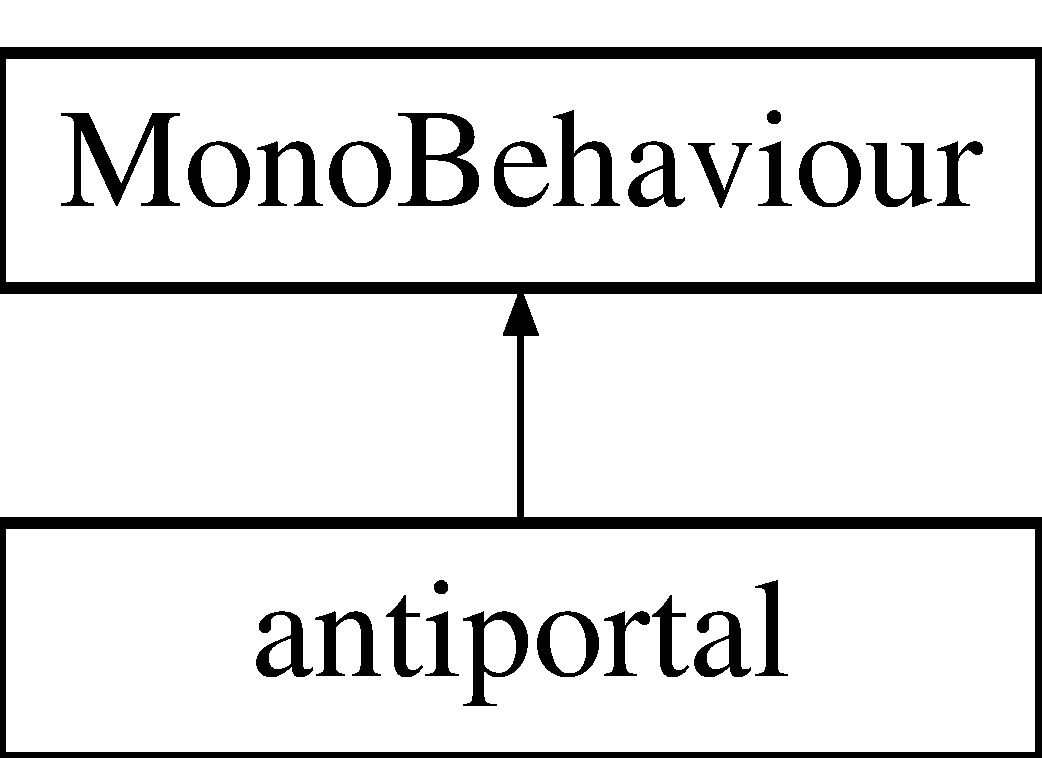
\includegraphics[height=2.000000cm]{classantiportal}
\end{center}
\end{figure}
\subsection*{Public Member Functions}
\begin{DoxyCompactItemize}
\item 
void \mbox{\hyperlink{classantiportal_a77c2fb6ea13c85d2edec17d01f0dfee4}{On\+Collision\+Enter2D}} (Collision2D collision)
\end{DoxyCompactItemize}


\subsection{Detailed Description}
Handles collision of portal bullet with terrain. 

\subsection{Member Function Documentation}
\mbox{\Hypertarget{classantiportal_a77c2fb6ea13c85d2edec17d01f0dfee4}\label{classantiportal_a77c2fb6ea13c85d2edec17d01f0dfee4}} 
\index{antiportal@{antiportal}!On\+Collision\+Enter2D@{On\+Collision\+Enter2D}}
\index{On\+Collision\+Enter2D@{On\+Collision\+Enter2D}!antiportal@{antiportal}}
\subsubsection{\texorpdfstring{On\+Collision\+Enter2\+D()}{OnCollisionEnter2D()}}
{\footnotesize\ttfamily void antiportal.\+On\+Collision\+Enter2D (\begin{DoxyParamCaption}\item[{Collision2D}]{collision }\end{DoxyParamCaption})\hspace{0.3cm}{\ttfamily [inline]}}

This method runs when the portal bullet hits a surface generating a collision. \begin{DoxyPrecond}{Precondition}
portal bullet is shot 
\end{DoxyPrecond}
\begin{DoxyPostcond}{Postcondition}
after collision bullet is removed but no portal is created. 
\end{DoxyPostcond}

\begin{DoxyParams}{Parameters}
{\em collision} & collision object created by the physics engine \\
\hline
\end{DoxyParams}


The documentation for this class was generated from the following file\+:\begin{DoxyCompactItemize}
\item 
Assets/\+Scripts/antiportal.\+cs\end{DoxyCompactItemize}

\hypertarget{class_box_movement}{}\section{Box\+Movement Class Reference}
\label{class_box_movement}\index{Box\+Movement@{Box\+Movement}}
Inheritance diagram for Box\+Movement\+:\begin{figure}[H]
\begin{center}
\leavevmode
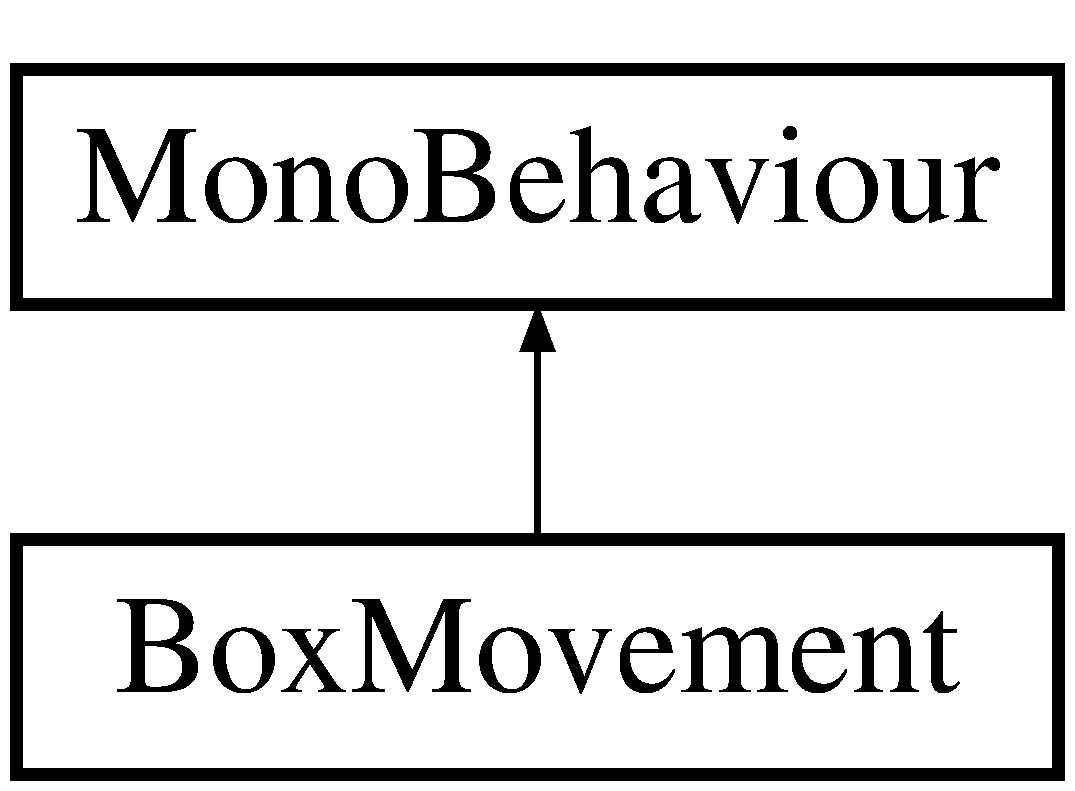
\includegraphics[height=2.000000cm]{class_box_movement}
\end{center}
\end{figure}
\subsection*{Public Member Functions}
\begin{DoxyCompactItemize}
\item 
\mbox{\Hypertarget{class_box_movement_a03b060c6c0cc28909fe9d197e0fd028a}\label{class_box_movement_a03b060c6c0cc28909fe9d197e0fd028a}} 
void {\bfseries Start} ()
\item 
void \mbox{\hyperlink{class_box_movement_ac523de4864d05c027a26c002feb0ddab}{Update}} ()
\end{DoxyCompactItemize}
\subsection*{Public Attributes}
\begin{DoxyCompactItemize}
\item 
\mbox{\Hypertarget{class_box_movement_ab093a3284a637c30339cd79b52dee4ed}\label{class_box_movement_ab093a3284a637c30339cd79b52dee4ed}} 
bool {\bfseries limitspeed} = true
\item 
\mbox{\Hypertarget{class_box_movement_a31cd8d25aebe904d30ae8b81fd987912}\label{class_box_movement_a31cd8d25aebe904d30ae8b81fd987912}} 
bool {\bfseries is\+Teleported} = false
\item 
\mbox{\Hypertarget{class_box_movement_a030be4c908d1ddf437002042704273f4}\label{class_box_movement_a030be4c908d1ddf437002042704273f4}} 
float {\bfseries current\+Speed} = 0f
\end{DoxyCompactItemize}


\subsection{Detailed Description}
Handles box movement. 

\subsection{Member Function Documentation}
\mbox{\Hypertarget{class_box_movement_ac523de4864d05c027a26c002feb0ddab}\label{class_box_movement_ac523de4864d05c027a26c002feb0ddab}} 
\index{Box\+Movement@{Box\+Movement}!Update@{Update}}
\index{Update@{Update}!Box\+Movement@{Box\+Movement}}
\subsubsection{\texorpdfstring{Update()}{Update()}}
{\footnotesize\ttfamily void Box\+Movement.\+Update (\begin{DoxyParamCaption}{ }\end{DoxyParamCaption})\hspace{0.3cm}{\ttfamily [inline]}}

Limits speed once grounded 

The documentation for this class was generated from the following file\+:\begin{DoxyCompactItemize}
\item 
Assets/\+Scripts/Box\+Movement.\+cs\end{DoxyCompactItemize}

\hypertarget{class_button}{}\section{Button Class Reference}
\label{class_button}\index{Button@{Button}}
Inheritance diagram for Button\+:\begin{figure}[H]
\begin{center}
\leavevmode
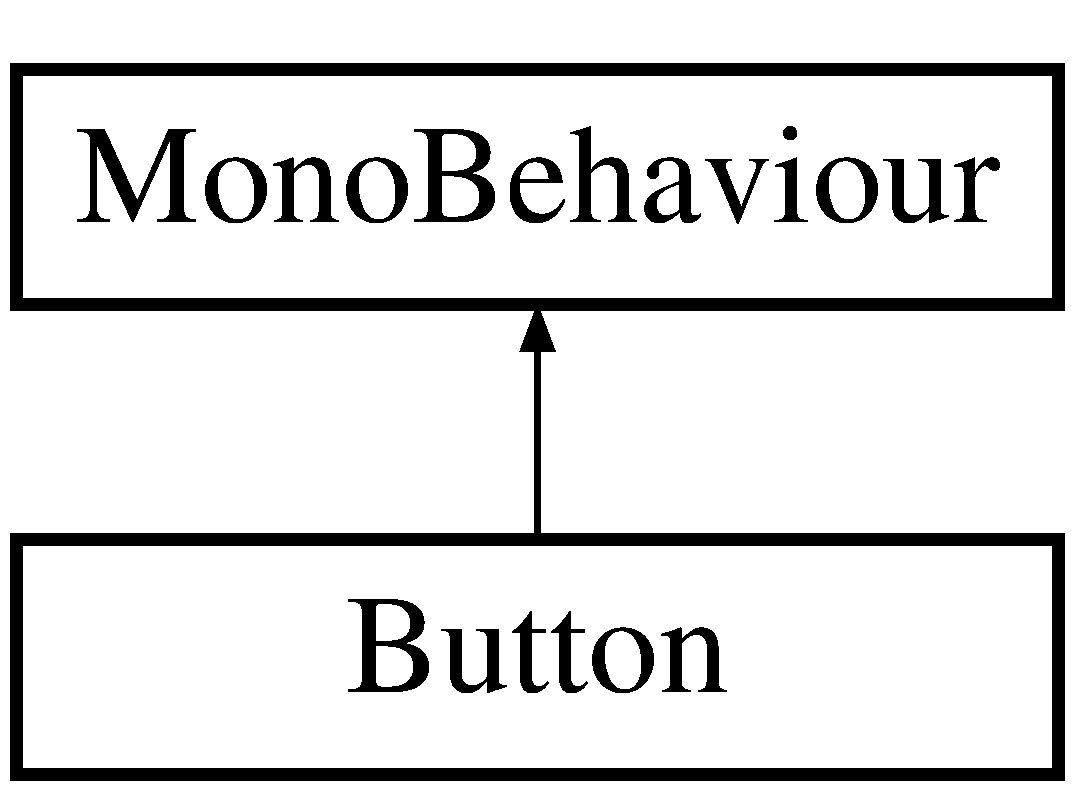
\includegraphics[height=2.000000cm]{class_button}
\end{center}
\end{figure}
\subsection*{Public Member Functions}
\begin{DoxyCompactItemize}
\item 
void \mbox{\hyperlink{class_button_a1ca1f623a8d5f7e9453eee7698e216ec}{Start}} ()
\item 
\mbox{\Hypertarget{class_button_abde2585e345c77634cc81b2f46c24936}\label{class_button_abde2585e345c77634cc81b2f46c24936}} 
void {\bfseries Update} ()
\end{DoxyCompactItemize}
\subsection*{Public Attributes}
\begin{DoxyCompactItemize}
\item 
\mbox{\Hypertarget{class_button_a6dff8f642d1cb675dbbca7fbe336850f}\label{class_button_a6dff8f642d1cb675dbbca7fbe336850f}} 
Game\+Object {\bfseries Button\+Pushed}
\item 
\mbox{\Hypertarget{class_button_a3fcbf5e728ccad68b7e80928ca8211f0}\label{class_button_a3fcbf5e728ccad68b7e80928ca8211f0}} 
Game\+Object {\bfseries Button\+Not\+Pushed}
\item 
\mbox{\Hypertarget{class_button_a1337709a1b2053148558e140ff59224b}\label{class_button_a1337709a1b2053148558e140ff59224b}} 
bool {\bfseries is\+Pushed} = false
\end{DoxyCompactItemize}


\subsection{Detailed Description}
Handles button pressing 

\subsection{Member Function Documentation}
\mbox{\Hypertarget{class_button_a1ca1f623a8d5f7e9453eee7698e216ec}\label{class_button_a1ca1f623a8d5f7e9453eee7698e216ec}} 
\index{Button@{Button}!Start@{Start}}
\index{Start@{Start}!Button@{Button}}
\subsubsection{\texorpdfstring{Start()}{Start()}}
{\footnotesize\ttfamily void Button.\+Start (\begin{DoxyParamCaption}{ }\end{DoxyParamCaption})\hspace{0.3cm}{\ttfamily [inline]}}

sets sprite to unpressed 

The documentation for this class was generated from the following file\+:\begin{DoxyCompactItemize}
\item 
Assets/\+Scripts/Button.\+cs\end{DoxyCompactItemize}

\hypertarget{classchip_a_i}{}\section{chip\+AI Class Reference}
\label{classchip_a_i}\index{chip\+AI@{chip\+AI}}
Inheritance diagram for chip\+AI\+:\begin{figure}[H]
\begin{center}
\leavevmode
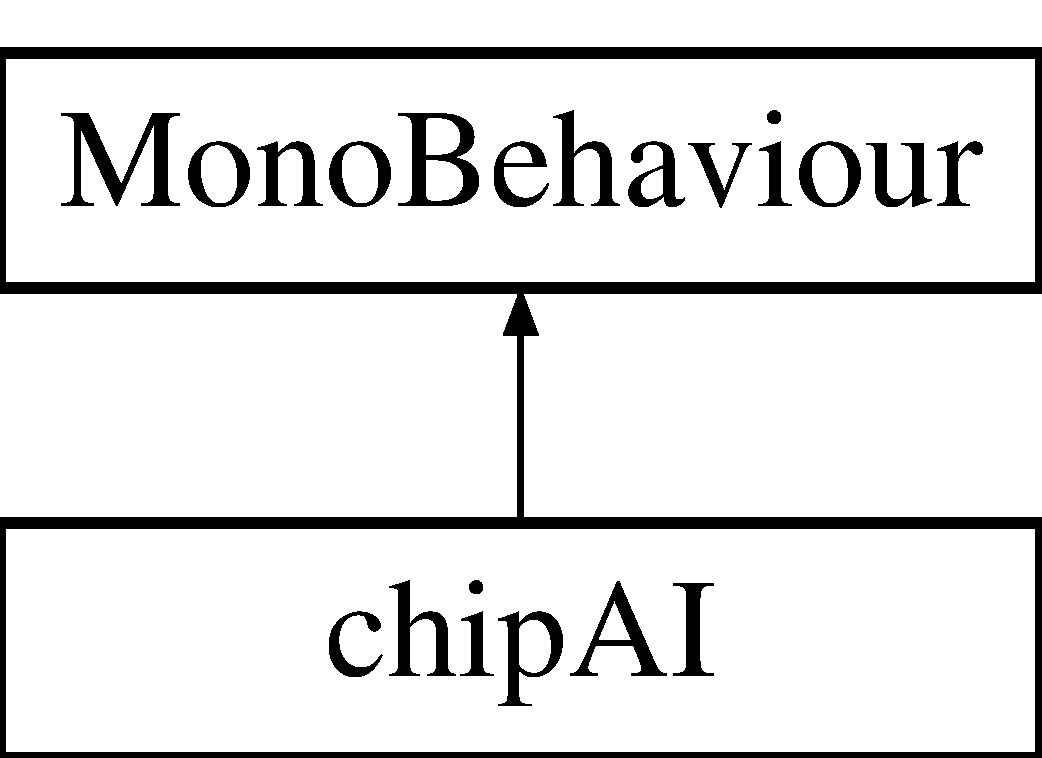
\includegraphics[height=2.000000cm]{classchip_a_i}
\end{center}
\end{figure}
\subsection*{Public Member Functions}
\begin{DoxyCompactItemize}
\item 
void \mbox{\hyperlink{classchip_a_i_ac18952b5af76d83063b05dae2e3c44c0}{Start}} ()
\item 
void \mbox{\hyperlink{classchip_a_i_a32e9caf3833a989c9b596bc9aa3bf0e9}{Update}} ()
\end{DoxyCompactItemize}
\subsection*{Public Attributes}
\begin{DoxyCompactItemize}
\item 
\mbox{\Hypertarget{classchip_a_i_a438b2bd6c24f4fa9af253b18a9910190}\label{classchip_a_i_a438b2bd6c24f4fa9af253b18a9910190}} 
Transform {\bfseries player}
\item 
\mbox{\Hypertarget{classchip_a_i_a7cb408dbc8e59270c802f7bac547d7df}\label{classchip_a_i_a7cb408dbc8e59270c802f7bac547d7df}} 
float {\bfseries speed} = 2f
\end{DoxyCompactItemize}


\subsection{Member Function Documentation}
\mbox{\Hypertarget{classchip_a_i_ac18952b5af76d83063b05dae2e3c44c0}\label{classchip_a_i_ac18952b5af76d83063b05dae2e3c44c0}} 
\index{chip\+AI@{chip\+AI}!Start@{Start}}
\index{Start@{Start}!chip\+AI@{chip\+AI}}
\subsubsection{\texorpdfstring{Start()}{Start()}}
{\footnotesize\ttfamily void chip\+A\+I.\+Start (\begin{DoxyParamCaption}{ }\end{DoxyParamCaption})\hspace{0.3cm}{\ttfamily [inline]}}

Sets player \mbox{\Hypertarget{classchip_a_i_a32e9caf3833a989c9b596bc9aa3bf0e9}\label{classchip_a_i_a32e9caf3833a989c9b596bc9aa3bf0e9}} 
\index{chip\+AI@{chip\+AI}!Update@{Update}}
\index{Update@{Update}!chip\+AI@{chip\+AI}}
\subsubsection{\texorpdfstring{Update()}{Update()}}
{\footnotesize\ttfamily void chip\+A\+I.\+Update (\begin{DoxyParamCaption}{ }\end{DoxyParamCaption})\hspace{0.3cm}{\ttfamily [inline]}}

Changes direction of chip toward player each frame. 

The documentation for this class was generated from the following file\+:\begin{DoxyCompactItemize}
\item 
Assets/\+Scripts/chip\+A\+I.\+cs\end{DoxyCompactItemize}

\hypertarget{class_collision_detection}{}\section{Collision\+Detection Class Reference}
\label{class_collision_detection}\index{Collision\+Detection@{Collision\+Detection}}
Inheritance diagram for Collision\+Detection\+:\begin{figure}[H]
\begin{center}
\leavevmode
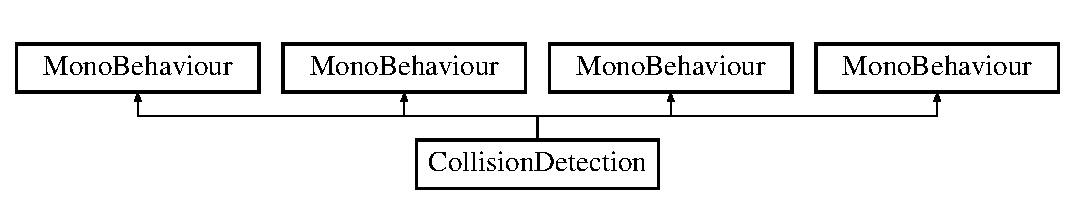
\includegraphics[height=2.000000cm]{class_collision_detection}
\end{center}
\end{figure}
\subsection*{Public Member Functions}
\begin{DoxyCompactItemize}
\item 
void \mbox{\hyperlink{class_collision_detection_ae5c7d4d990b3c888dc8866821a3d0366}{On\+Collision\+Enter2D}} (Collision2D collision)
\item 
void \mbox{\hyperlink{class_collision_detection_ae5c7d4d990b3c888dc8866821a3d0366}{On\+Collision\+Enter2D}} (Collision2D collision)
\end{DoxyCompactItemize}
\subsection*{Public Attributes}
\begin{DoxyCompactItemize}
\item 
\mbox{\Hypertarget{class_collision_detection_a5998d298c2f3c52ca58af7e2604a8559}\label{class_collision_detection_a5998d298c2f3c52ca58af7e2604a8559}} 
Game\+Object {\bfseries blue\+Portal}
\item 
\mbox{\Hypertarget{class_collision_detection_acb663162929e709c69b80cf62f864d6a}\label{class_collision_detection_acb663162929e709c69b80cf62f864d6a}} 
Game\+Object {\bfseries red\+Portal}
\item 
\mbox{\Hypertarget{class_collision_detection_a4bd58b38fd8034d725f0262c78addfeb}\label{class_collision_detection_a4bd58b38fd8034d725f0262c78addfeb}} 
Game\+Object {\bfseries Portal}
\item 
\mbox{\Hypertarget{class_collision_detection_a4281fd2d4607ab7b94d947928dc388a9}\label{class_collision_detection_a4281fd2d4607ab7b94d947928dc388a9}} 
Game\+Object {\bfseries New\+Portal}
\end{DoxyCompactItemize}


\subsection{Detailed Description}
Handles collision of portal bullet with terrain. 

\subsection{Member Function Documentation}
\mbox{\Hypertarget{class_collision_detection_ae5c7d4d990b3c888dc8866821a3d0366}\label{class_collision_detection_ae5c7d4d990b3c888dc8866821a3d0366}} 
\index{Collision\+Detection@{Collision\+Detection}!On\+Collision\+Enter2D@{On\+Collision\+Enter2D}}
\index{On\+Collision\+Enter2D@{On\+Collision\+Enter2D}!Collision\+Detection@{Collision\+Detection}}
\subsubsection{\texorpdfstring{On\+Collision\+Enter2\+D()}{OnCollisionEnter2D()}\hspace{0.1cm}{\footnotesize\ttfamily [1/2]}}
{\footnotesize\ttfamily void Collision\+Detection.\+On\+Collision\+Enter2D (\begin{DoxyParamCaption}\item[{Collision2D}]{collision }\end{DoxyParamCaption})\hspace{0.3cm}{\ttfamily [inline]}}

This method runs when the portal bullet hits a surface generating a collision. \begin{DoxyPrecond}{Precondition}
portal bullet is shot 
\end{DoxyPrecond}
\begin{DoxyPostcond}{Postcondition}
after collision with appropriate surface portal gets created and previous portal gets destroyed 
\end{DoxyPostcond}
\mbox{\Hypertarget{class_collision_detection_ae5c7d4d990b3c888dc8866821a3d0366}\label{class_collision_detection_ae5c7d4d990b3c888dc8866821a3d0366}} 
\index{Collision\+Detection@{Collision\+Detection}!On\+Collision\+Enter2D@{On\+Collision\+Enter2D}}
\index{On\+Collision\+Enter2D@{On\+Collision\+Enter2D}!Collision\+Detection@{Collision\+Detection}}
\subsubsection{\texorpdfstring{On\+Collision\+Enter2\+D()}{OnCollisionEnter2D()}\hspace{0.1cm}{\footnotesize\ttfamily [2/2]}}
{\footnotesize\ttfamily void Collision\+Detection.\+On\+Collision\+Enter2D (\begin{DoxyParamCaption}\item[{Collision2D}]{collision }\end{DoxyParamCaption})\hspace{0.3cm}{\ttfamily [inline]}}

This method runs when the portal bullet hits a surface generating a collision. \begin{DoxyPrecond}{Precondition}
portal bullet is shot 
\end{DoxyPrecond}
\begin{DoxyPostcond}{Postcondition}
after collision with appropriate surface portal gets created and previous portal gets destroyed 
\end{DoxyPostcond}

\begin{DoxyParams}{Parameters}
{\em collision} & collision object created by the physics engine \\
\hline
\end{DoxyParams}


The documentation for this class was generated from the following file\+:\begin{DoxyCompactItemize}
\item 
Assets/\+Scripts/Collision\+Detection.\+cs\end{DoxyCompactItemize}

\hypertarget{class_game_manager}{}\section{Game\+Manager Class Reference}
\label{class_game_manager}\index{Game\+Manager@{Game\+Manager}}
Inheritance diagram for Game\+Manager\+:\begin{figure}[H]
\begin{center}
\leavevmode
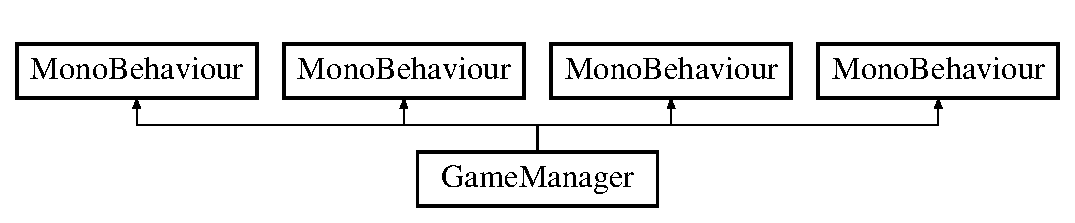
\includegraphics[height=2.000000cm]{class_game_manager}
\end{center}
\end{figure}
\subsection*{Public Member Functions}
\begin{DoxyCompactItemize}
\item 
void \mbox{\hyperlink{class_game_manager_a5ccfacd027ad08eeb4ff1f25a7f59c98}{Start}} ()
\item 
void \mbox{\hyperlink{class_game_manager_a76a27f36d082e328bd1c7748d8832816}{Win}} ()
\end{DoxyCompactItemize}
\subsection*{Public Attributes}
\begin{DoxyCompactItemize}
\item 
\mbox{\Hypertarget{class_game_manager_a9e2addf3b88748a4d46a5428e1e332f0}\label{class_game_manager_a9e2addf3b88748a4d46a5428e1e332f0}} 
Game\+Object {\bfseries you\+Win}
\end{DoxyCompactItemize}
\subsection*{Static Public Attributes}
\begin{DoxyCompactItemize}
\item 
\mbox{\Hypertarget{class_game_manager_a7666e8468dac197b9eb32dd32128524f}\label{class_game_manager_a7666e8468dac197b9eb32dd32128524f}} 
static \mbox{\hyperlink{class_game_manager}{Game\+Manager}} {\bfseries instance} = null
\end{DoxyCompactItemize}


\subsection{Detailed Description}
Handles game instance. 

\subsection{Member Function Documentation}
\mbox{\Hypertarget{class_game_manager_a5ccfacd027ad08eeb4ff1f25a7f59c98}\label{class_game_manager_a5ccfacd027ad08eeb4ff1f25a7f59c98}} 
\index{Game\+Manager@{Game\+Manager}!Start@{Start}}
\index{Start@{Start}!Game\+Manager@{Game\+Manager}}
\subsubsection{\texorpdfstring{Start()}{Start()}}
{\footnotesize\ttfamily void Game\+Manager.\+Start (\begin{DoxyParamCaption}{ }\end{DoxyParamCaption})\hspace{0.3cm}{\ttfamily [inline]}}

Runs at start. \begin{DoxyPrecond}{Precondition}
game starts 
\end{DoxyPrecond}
\begin{DoxyPostcond}{Postcondition}
Instance of the game is created 
\end{DoxyPostcond}
\mbox{\Hypertarget{class_game_manager_a76a27f36d082e328bd1c7748d8832816}\label{class_game_manager_a76a27f36d082e328bd1c7748d8832816}} 
\index{Game\+Manager@{Game\+Manager}!Win@{Win}}
\index{Win@{Win}!Game\+Manager@{Game\+Manager}}
\subsubsection{\texorpdfstring{Win()}{Win()}}
{\footnotesize\ttfamily void Game\+Manager.\+Win (\begin{DoxyParamCaption}{ }\end{DoxyParamCaption})\hspace{0.3cm}{\ttfamily [inline]}}

Sets win state to true. function is called by \mbox{\hyperlink{class_win_game}{Win\+Game()}} \begin{DoxyPrecond}{Precondition}
User reached door object 
\end{DoxyPrecond}
\begin{DoxyPostcond}{Postcondition}
Success message is displayed 
\end{DoxyPostcond}


The documentation for this class was generated from the following file\+:\begin{DoxyCompactItemize}
\item 
Assets/\+Scripts/Game\+Manager.\+cs\end{DoxyCompactItemize}

\hypertarget{class_gun_rotation}{}\section{Gun\+Rotation Class Reference}
\label{class_gun_rotation}\index{Gun\+Rotation@{Gun\+Rotation}}
Inheritance diagram for Gun\+Rotation\+:\begin{figure}[H]
\begin{center}
\leavevmode
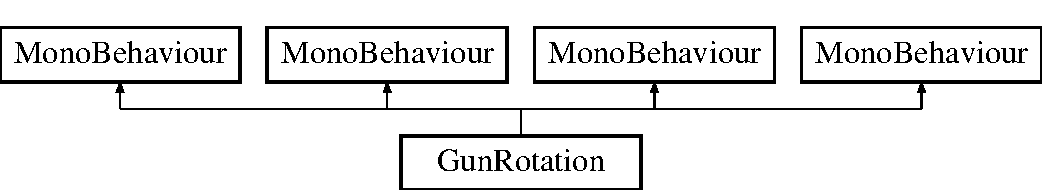
\includegraphics[height=2.000000cm]{class_gun_rotation}
\end{center}
\end{figure}


\subsection{Detailed Description}
Aims gun at mouse cursor. 

The documentation for this class was generated from the following file\+:\begin{DoxyCompactItemize}
\item 
Assets/\+Scripts/Gun\+Rotation.\+cs\end{DoxyCompactItemize}

\hypertarget{classhazard}{}\section{hazard Class Reference}
\label{classhazard}\index{hazard@{hazard}}
Inheritance diagram for hazard\+:\begin{figure}[H]
\begin{center}
\leavevmode
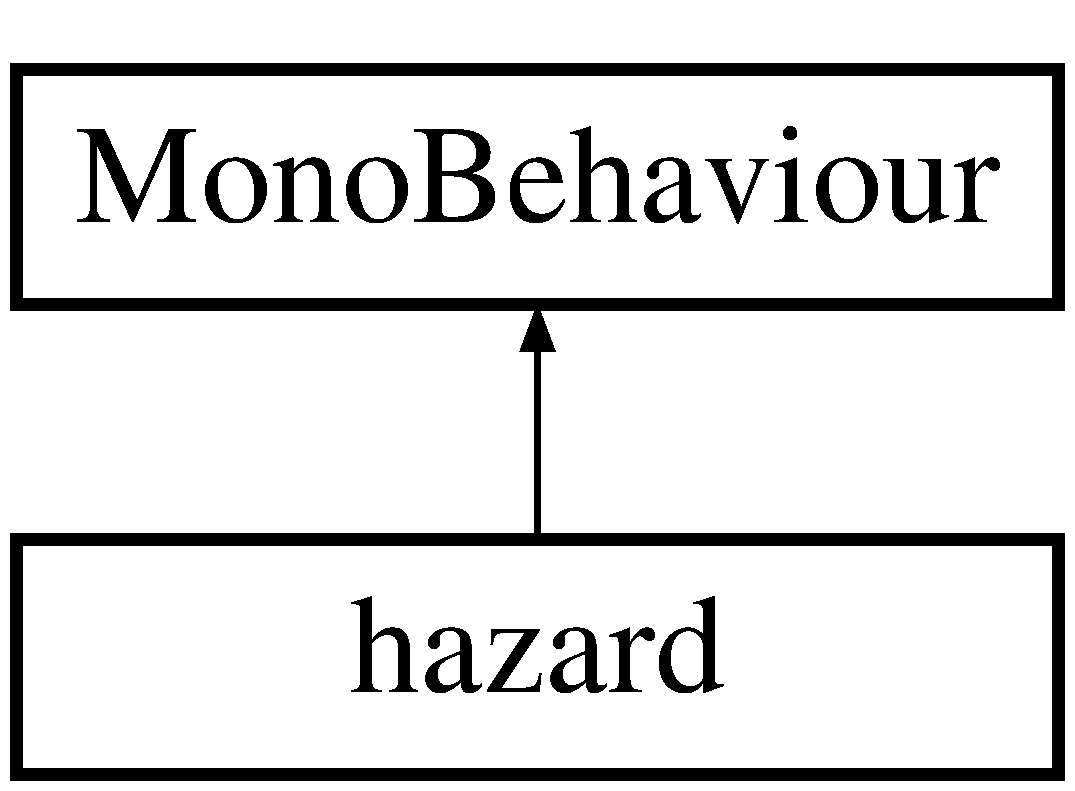
\includegraphics[height=2.000000cm]{classhazard}
\end{center}
\end{figure}
\subsection*{Public Member Functions}
\begin{DoxyCompactItemize}
\item 
void \mbox{\hyperlink{classhazard_a8ad9f65467a60d2379e1b879568f9703}{On\+Collision\+Enter2D}} (Collision2D collision)
\end{DoxyCompactItemize}


\subsection{Detailed Description}
Handles collision with enemies or red platforms 

\subsection{Member Function Documentation}
\mbox{\Hypertarget{classhazard_a8ad9f65467a60d2379e1b879568f9703}\label{classhazard_a8ad9f65467a60d2379e1b879568f9703}} 
\index{hazard@{hazard}!On\+Collision\+Enter2D@{On\+Collision\+Enter2D}}
\index{On\+Collision\+Enter2D@{On\+Collision\+Enter2D}!hazard@{hazard}}
\subsubsection{\texorpdfstring{On\+Collision\+Enter2\+D()}{OnCollisionEnter2D()}}
{\footnotesize\ttfamily void hazard.\+On\+Collision\+Enter2D (\begin{DoxyParamCaption}\item[{Collision2D}]{collision }\end{DoxyParamCaption})\hspace{0.3cm}{\ttfamily [inline]}}

Restarts level upon collision 
\begin{DoxyParams}{Parameters}
{\em collision} & collision object created by the physics engine \\
\hline
\end{DoxyParams}


The documentation for this class was generated from the following file\+:\begin{DoxyCompactItemize}
\item 
Assets/\+Scripts/hazard.\+cs\end{DoxyCompactItemize}

\hypertarget{class_level_selector}{}\section{Level\+Selector Class Reference}
\label{class_level_selector}\index{Level\+Selector@{Level\+Selector}}
Inheritance diagram for Level\+Selector\+:\begin{figure}[H]
\begin{center}
\leavevmode
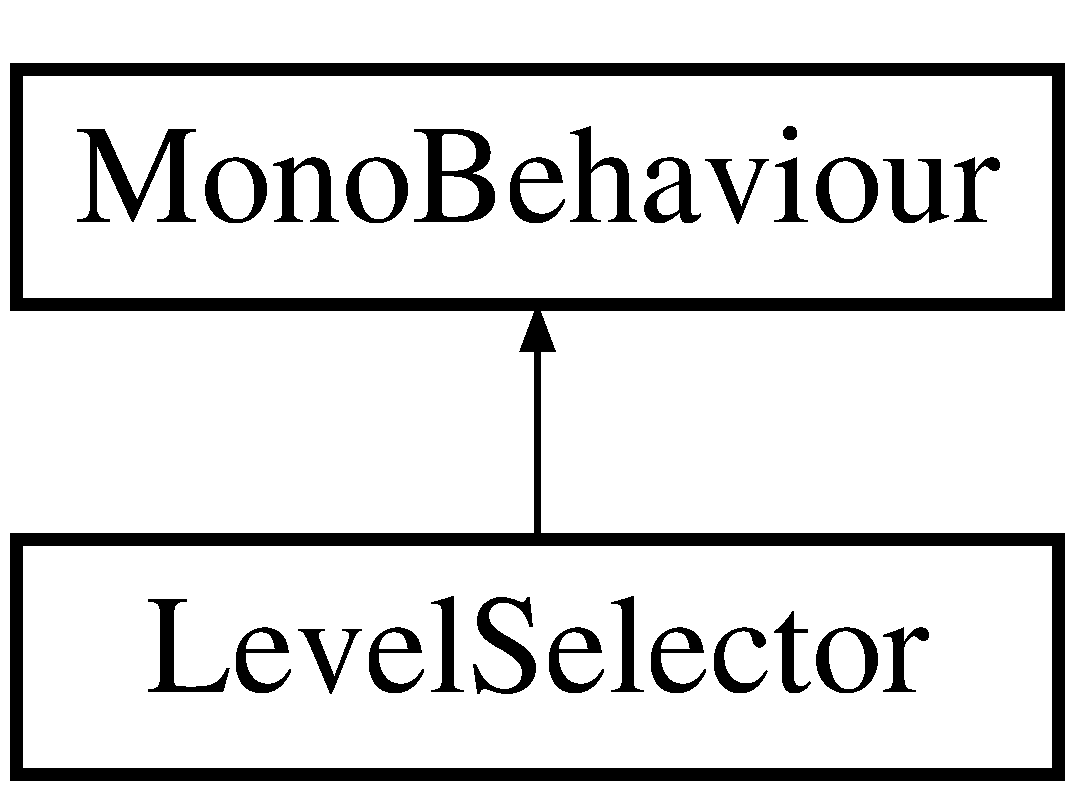
\includegraphics[height=2.000000cm]{class_level_selector}
\end{center}
\end{figure}
\subsection*{Public Member Functions}
\begin{DoxyCompactItemize}
\item 
void \mbox{\hyperlink{class_level_selector_a9f5a0a4de4a6d9fbec81ed65cc0f7728}{Level1}} ()
\item 
void \mbox{\hyperlink{class_level_selector_adeb0b4be0958981b1a1a5a620361bc30}{Level2}} ()
\item 
void \mbox{\hyperlink{class_level_selector_a5dfc03a08d600ba73bdd2de47782d3d0}{Level3}} ()
\item 
void \mbox{\hyperlink{class_level_selector_aa2a04a7aabb5008cc36cadef9921e10b}{Level4}} ()
\item 
void \mbox{\hyperlink{class_level_selector_a3cbc0621c0e2c2533ee6be55bab1e519}{Level5}} ()
\item 
void \mbox{\hyperlink{class_level_selector_a9b7572b24c4f628e31bb4a0d4d35dfee}{Level6}} ()
\item 
void \mbox{\hyperlink{class_level_selector_a85b373b055b331c885add13d097251d5}{Level7}} ()
\item 
void \mbox{\hyperlink{class_level_selector_a902e7d01b59f6c6affb89c28c9529a88}{Level8}} ()
\item 
void \mbox{\hyperlink{class_level_selector_a8be23d6e76b3eaf708f2ddeb733addac}{Level9}} ()
\item 
void \mbox{\hyperlink{class_level_selector_a3fe4d7253904b5b7556aa52401136b45}{Menu}} ()
\end{DoxyCompactItemize}


\subsection{Detailed Description}
Handles switching between levels and main menu 

\subsection{Member Function Documentation}
\mbox{\Hypertarget{class_level_selector_a9f5a0a4de4a6d9fbec81ed65cc0f7728}\label{class_level_selector_a9f5a0a4de4a6d9fbec81ed65cc0f7728}} 
\index{Level\+Selector@{Level\+Selector}!Level1@{Level1}}
\index{Level1@{Level1}!Level\+Selector@{Level\+Selector}}
\subsubsection{\texorpdfstring{Level1()}{Level1()}}
{\footnotesize\ttfamily void Level\+Selector.\+Level1 (\begin{DoxyParamCaption}{ }\end{DoxyParamCaption})\hspace{0.3cm}{\ttfamily [inline]}}

Changes scene to level 1 \mbox{\Hypertarget{class_level_selector_adeb0b4be0958981b1a1a5a620361bc30}\label{class_level_selector_adeb0b4be0958981b1a1a5a620361bc30}} 
\index{Level\+Selector@{Level\+Selector}!Level2@{Level2}}
\index{Level2@{Level2}!Level\+Selector@{Level\+Selector}}
\subsubsection{\texorpdfstring{Level2()}{Level2()}}
{\footnotesize\ttfamily void Level\+Selector.\+Level2 (\begin{DoxyParamCaption}{ }\end{DoxyParamCaption})\hspace{0.3cm}{\ttfamily [inline]}}

Changes scene to level 2 \mbox{\Hypertarget{class_level_selector_a5dfc03a08d600ba73bdd2de47782d3d0}\label{class_level_selector_a5dfc03a08d600ba73bdd2de47782d3d0}} 
\index{Level\+Selector@{Level\+Selector}!Level3@{Level3}}
\index{Level3@{Level3}!Level\+Selector@{Level\+Selector}}
\subsubsection{\texorpdfstring{Level3()}{Level3()}}
{\footnotesize\ttfamily void Level\+Selector.\+Level3 (\begin{DoxyParamCaption}{ }\end{DoxyParamCaption})\hspace{0.3cm}{\ttfamily [inline]}}

Changes scene to level 3 \mbox{\Hypertarget{class_level_selector_aa2a04a7aabb5008cc36cadef9921e10b}\label{class_level_selector_aa2a04a7aabb5008cc36cadef9921e10b}} 
\index{Level\+Selector@{Level\+Selector}!Level4@{Level4}}
\index{Level4@{Level4}!Level\+Selector@{Level\+Selector}}
\subsubsection{\texorpdfstring{Level4()}{Level4()}}
{\footnotesize\ttfamily void Level\+Selector.\+Level4 (\begin{DoxyParamCaption}{ }\end{DoxyParamCaption})\hspace{0.3cm}{\ttfamily [inline]}}

Changes scene to level 4 \mbox{\Hypertarget{class_level_selector_a3cbc0621c0e2c2533ee6be55bab1e519}\label{class_level_selector_a3cbc0621c0e2c2533ee6be55bab1e519}} 
\index{Level\+Selector@{Level\+Selector}!Level5@{Level5}}
\index{Level5@{Level5}!Level\+Selector@{Level\+Selector}}
\subsubsection{\texorpdfstring{Level5()}{Level5()}}
{\footnotesize\ttfamily void Level\+Selector.\+Level5 (\begin{DoxyParamCaption}{ }\end{DoxyParamCaption})\hspace{0.3cm}{\ttfamily [inline]}}

Changes scene to level 5 \mbox{\Hypertarget{class_level_selector_a9b7572b24c4f628e31bb4a0d4d35dfee}\label{class_level_selector_a9b7572b24c4f628e31bb4a0d4d35dfee}} 
\index{Level\+Selector@{Level\+Selector}!Level6@{Level6}}
\index{Level6@{Level6}!Level\+Selector@{Level\+Selector}}
\subsubsection{\texorpdfstring{Level6()}{Level6()}}
{\footnotesize\ttfamily void Level\+Selector.\+Level6 (\begin{DoxyParamCaption}{ }\end{DoxyParamCaption})\hspace{0.3cm}{\ttfamily [inline]}}

Changes scene to level 6 \mbox{\Hypertarget{class_level_selector_a85b373b055b331c885add13d097251d5}\label{class_level_selector_a85b373b055b331c885add13d097251d5}} 
\index{Level\+Selector@{Level\+Selector}!Level7@{Level7}}
\index{Level7@{Level7}!Level\+Selector@{Level\+Selector}}
\subsubsection{\texorpdfstring{Level7()}{Level7()}}
{\footnotesize\ttfamily void Level\+Selector.\+Level7 (\begin{DoxyParamCaption}{ }\end{DoxyParamCaption})\hspace{0.3cm}{\ttfamily [inline]}}

Changes scene to level 7 \mbox{\Hypertarget{class_level_selector_a902e7d01b59f6c6affb89c28c9529a88}\label{class_level_selector_a902e7d01b59f6c6affb89c28c9529a88}} 
\index{Level\+Selector@{Level\+Selector}!Level8@{Level8}}
\index{Level8@{Level8}!Level\+Selector@{Level\+Selector}}
\subsubsection{\texorpdfstring{Level8()}{Level8()}}
{\footnotesize\ttfamily void Level\+Selector.\+Level8 (\begin{DoxyParamCaption}{ }\end{DoxyParamCaption})\hspace{0.3cm}{\ttfamily [inline]}}

Changes scene to level 8 \mbox{\Hypertarget{class_level_selector_a8be23d6e76b3eaf708f2ddeb733addac}\label{class_level_selector_a8be23d6e76b3eaf708f2ddeb733addac}} 
\index{Level\+Selector@{Level\+Selector}!Level9@{Level9}}
\index{Level9@{Level9}!Level\+Selector@{Level\+Selector}}
\subsubsection{\texorpdfstring{Level9()}{Level9()}}
{\footnotesize\ttfamily void Level\+Selector.\+Level9 (\begin{DoxyParamCaption}{ }\end{DoxyParamCaption})\hspace{0.3cm}{\ttfamily [inline]}}

Changes scene to level 9 \mbox{\Hypertarget{class_level_selector_a3fe4d7253904b5b7556aa52401136b45}\label{class_level_selector_a3fe4d7253904b5b7556aa52401136b45}} 
\index{Level\+Selector@{Level\+Selector}!Menu@{Menu}}
\index{Menu@{Menu}!Level\+Selector@{Level\+Selector}}
\subsubsection{\texorpdfstring{Menu()}{Menu()}}
{\footnotesize\ttfamily void Level\+Selector.\+Menu (\begin{DoxyParamCaption}{ }\end{DoxyParamCaption})\hspace{0.3cm}{\ttfamily [inline]}}

Changes scene to main menu 

The documentation for this class was generated from the following file\+:\begin{DoxyCompactItemize}
\item 
Assets/\+Scripts/Level\+Selector.\+cs\end{DoxyCompactItemize}

\hypertarget{class_main_menu}{}\section{Main\+Menu Class Reference}
\label{class_main_menu}\index{Main\+Menu@{Main\+Menu}}
Inheritance diagram for Main\+Menu\+:\begin{figure}[H]
\begin{center}
\leavevmode
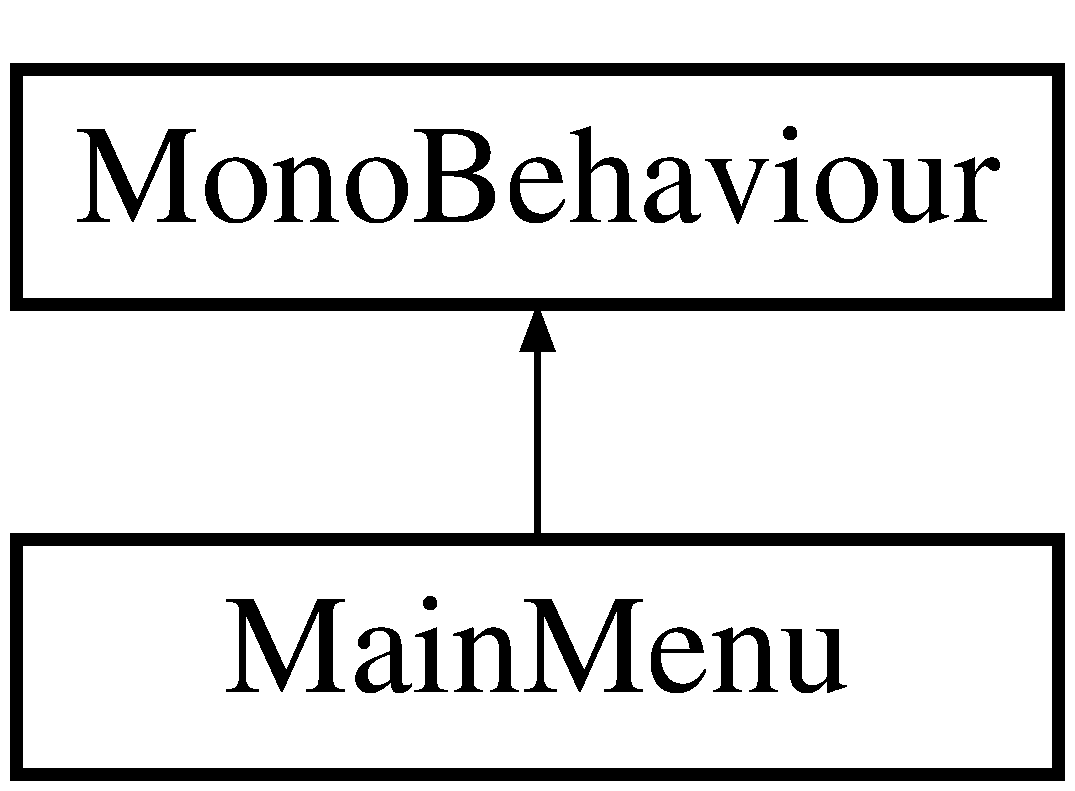
\includegraphics[height=2.000000cm]{class_main_menu}
\end{center}
\end{figure}
\subsection*{Public Member Functions}
\begin{DoxyCompactItemize}
\item 
void \mbox{\hyperlink{class_main_menu_a18b84d06aaaeb1086349846809d31ab3}{Play}} ()
\item 
void \mbox{\hyperlink{class_main_menu_a7b541911775a290b2f3b4b22db4b830a}{Levels}} ()
\item 
void \mbox{\hyperlink{class_main_menu_a8c08f64fe9eb1b70fb787c0215bd1023}{Test}} ()
\item 
void \mbox{\hyperlink{class_main_menu_a485db7cf60c0b93ecc87b9273bcce78b}{Quit\+Game}} ()
\end{DoxyCompactItemize}


\subsection{Detailed Description}
Main menu functionality 

\subsection{Member Function Documentation}
\mbox{\Hypertarget{class_main_menu_a7b541911775a290b2f3b4b22db4b830a}\label{class_main_menu_a7b541911775a290b2f3b4b22db4b830a}} 
\index{Main\+Menu@{Main\+Menu}!Levels@{Levels}}
\index{Levels@{Levels}!Main\+Menu@{Main\+Menu}}
\subsubsection{\texorpdfstring{Levels()}{Levels()}}
{\footnotesize\ttfamily void Main\+Menu.\+Levels (\begin{DoxyParamCaption}{ }\end{DoxyParamCaption})\hspace{0.3cm}{\ttfamily [inline]}}

Changes scene to level select screen \mbox{\Hypertarget{class_main_menu_a18b84d06aaaeb1086349846809d31ab3}\label{class_main_menu_a18b84d06aaaeb1086349846809d31ab3}} 
\index{Main\+Menu@{Main\+Menu}!Play@{Play}}
\index{Play@{Play}!Main\+Menu@{Main\+Menu}}
\subsubsection{\texorpdfstring{Play()}{Play()}}
{\footnotesize\ttfamily void Main\+Menu.\+Play (\begin{DoxyParamCaption}{ }\end{DoxyParamCaption})\hspace{0.3cm}{\ttfamily [inline]}}

Begins level 1 \mbox{\Hypertarget{class_main_menu_a485db7cf60c0b93ecc87b9273bcce78b}\label{class_main_menu_a485db7cf60c0b93ecc87b9273bcce78b}} 
\index{Main\+Menu@{Main\+Menu}!Quit\+Game@{Quit\+Game}}
\index{Quit\+Game@{Quit\+Game}!Main\+Menu@{Main\+Menu}}
\subsubsection{\texorpdfstring{Quit\+Game()}{QuitGame()}}
{\footnotesize\ttfamily void Main\+Menu.\+Quit\+Game (\begin{DoxyParamCaption}{ }\end{DoxyParamCaption})\hspace{0.3cm}{\ttfamily [inline]}}

Exits game \mbox{\Hypertarget{class_main_menu_a8c08f64fe9eb1b70fb787c0215bd1023}\label{class_main_menu_a8c08f64fe9eb1b70fb787c0215bd1023}} 
\index{Main\+Menu@{Main\+Menu}!Test@{Test}}
\index{Test@{Test}!Main\+Menu@{Main\+Menu}}
\subsubsection{\texorpdfstring{Test()}{Test()}}
{\footnotesize\ttfamily void Main\+Menu.\+Test (\begin{DoxyParamCaption}{ }\end{DoxyParamCaption})\hspace{0.3cm}{\ttfamily [inline]}}

Changes to testing scene 

The documentation for this class was generated from the following file\+:\begin{DoxyCompactItemize}
\item 
Assets/\+Scripts/Main\+Menu.\+cs\end{DoxyCompactItemize}

\hypertarget{classopen___door}{}\section{open\+\_\+\+Door Class Reference}
\label{classopen___door}\index{open\+\_\+\+Door@{open\+\_\+\+Door}}
Inheritance diagram for open\+\_\+\+Door\+:\begin{figure}[H]
\begin{center}
\leavevmode
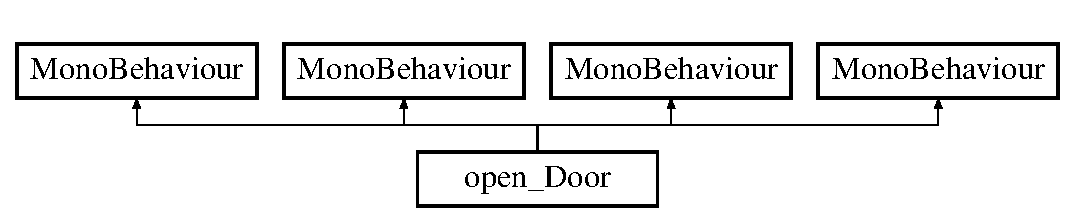
\includegraphics[height=2.000000cm]{classopen___door}
\end{center}
\end{figure}
\subsection*{Public Member Functions}
\begin{DoxyCompactItemize}
\item 
\mbox{\Hypertarget{classopen___door_a73d16144fb87c086186bd5c26b5919a5}\label{classopen___door_a73d16144fb87c086186bd5c26b5919a5}} 
void {\bfseries Start} ()
\item 
\mbox{\Hypertarget{classopen___door_a7689f551c5c3a63718e506e6e101c36f}\label{classopen___door_a7689f551c5c3a63718e506e6e101c36f}} 
void {\bfseries Update} ()
\item 
void \mbox{\hyperlink{classopen___door_af445b9df0f862ee2c2d667d6b1f92811}{player\+Hits\+Door}} (Collision2D collision)
\end{DoxyCompactItemize}
\subsection*{Public Attributes}
\begin{DoxyCompactItemize}
\item 
\mbox{\Hypertarget{classopen___door_afdfd02e742a29a8091cc062da7ebf335}\label{classopen___door_afdfd02e742a29a8091cc062da7ebf335}} 
bool {\bfseries door\+Is\+Open} = false
\item 
\mbox{\Hypertarget{classopen___door_a2d7b03a65ed29ef63bd7d17a19b57404}\label{classopen___door_a2d7b03a65ed29ef63bd7d17a19b57404}} 
Game\+Object {\bfseries Door}
\end{DoxyCompactItemize}


\subsection{Detailed Description}
Opens final door. 

\subsection{Member Function Documentation}
\mbox{\Hypertarget{classopen___door_af445b9df0f862ee2c2d667d6b1f92811}\label{classopen___door_af445b9df0f862ee2c2d667d6b1f92811}} 
\index{open\+\_\+\+Door@{open\+\_\+\+Door}!player\+Hits\+Door@{player\+Hits\+Door}}
\index{player\+Hits\+Door@{player\+Hits\+Door}!open\+\_\+\+Door@{open\+\_\+\+Door}}
\subsubsection{\texorpdfstring{player\+Hits\+Door()}{playerHitsDoor()}}
{\footnotesize\ttfamily void open\+\_\+\+Door.\+player\+Hits\+Door (\begin{DoxyParamCaption}\item[{Collision2D}]{collision }\end{DoxyParamCaption})\hspace{0.3cm}{\ttfamily [inline]}}

will start animation after player collides with exit door indicating level was completed. 

The documentation for this class was generated from the following file\+:\begin{DoxyCompactItemize}
\item 
Assets/\+Scripts/open\+\_\+\+Door.\+cs\end{DoxyCompactItemize}

\hypertarget{class_pause}{}\section{Pause Class Reference}
\label{class_pause}\index{Pause@{Pause}}
Inheritance diagram for Pause\+:\begin{figure}[H]
\begin{center}
\leavevmode
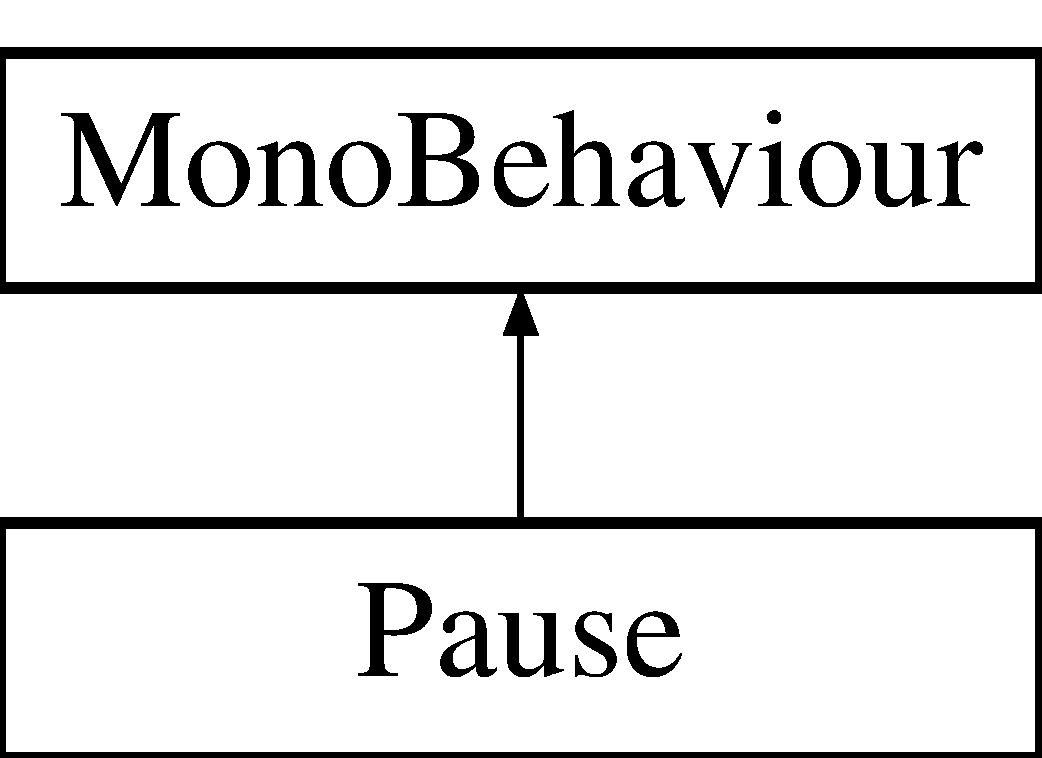
\includegraphics[height=2.000000cm]{class_pause}
\end{center}
\end{figure}
\subsection*{Public Member Functions}
\begin{DoxyCompactItemize}
\item 
void \mbox{\hyperlink{class_pause_a2676d511f741a690dd8a1d6f64aef89c}{Start}} ()
\item 
void \mbox{\hyperlink{class_pause_aab062f8945cc0bad08b554ad58357dc5}{Update}} ()
\item 
void \mbox{\hyperlink{class_pause_a7c2e0304ced82527cf7f676c92b16a7c}{On\+G\+UI}} ()
\end{DoxyCompactItemize}
\subsection*{Public Attributes}
\begin{DoxyCompactItemize}
\item 
\mbox{\Hypertarget{class_pause_aa5274c1fe482791dd670f1db1ec19600}\label{class_pause_aa5274c1fe482791dd670f1db1ec19600}} 
bool {\bfseries paused}
\end{DoxyCompactItemize}


\subsection{Detailed Description}
Pauses the game and adds menu options 

\subsection{Member Function Documentation}
\mbox{\Hypertarget{class_pause_a7c2e0304ced82527cf7f676c92b16a7c}\label{class_pause_a7c2e0304ced82527cf7f676c92b16a7c}} 
\index{Pause@{Pause}!On\+G\+UI@{On\+G\+UI}}
\index{On\+G\+UI@{On\+G\+UI}!Pause@{Pause}}
\subsubsection{\texorpdfstring{On\+G\+U\+I()}{OnGUI()}}
{\footnotesize\ttfamily void Pause.\+On\+G\+UI (\begin{DoxyParamCaption}{ }\end{DoxyParamCaption})\hspace{0.3cm}{\ttfamily [inline]}}

Displays pause menu \mbox{\Hypertarget{class_pause_a2676d511f741a690dd8a1d6f64aef89c}\label{class_pause_a2676d511f741a690dd8a1d6f64aef89c}} 
\index{Pause@{Pause}!Start@{Start}}
\index{Start@{Start}!Pause@{Pause}}
\subsubsection{\texorpdfstring{Start()}{Start()}}
{\footnotesize\ttfamily void Pause.\+Start (\begin{DoxyParamCaption}{ }\end{DoxyParamCaption})\hspace{0.3cm}{\ttfamily [inline]}}

Sets paused state to false \mbox{\Hypertarget{class_pause_aab062f8945cc0bad08b554ad58357dc5}\label{class_pause_aab062f8945cc0bad08b554ad58357dc5}} 
\index{Pause@{Pause}!Update@{Update}}
\index{Update@{Update}!Pause@{Pause}}
\subsubsection{\texorpdfstring{Update()}{Update()}}
{\footnotesize\ttfamily void Pause.\+Update (\begin{DoxyParamCaption}{ }\end{DoxyParamCaption})\hspace{0.3cm}{\ttfamily [inline]}}

Checks for esc key press, then pauses or unpauses if it is 

The documentation for this class was generated from the following file\+:\begin{DoxyCompactItemize}
\item 
Assets/\+Scripts/Pause.\+cs\end{DoxyCompactItemize}

\hypertarget{class_player_movement}{}\section{Player\+Movement Class Reference}
\label{class_player_movement}\index{Player\+Movement@{Player\+Movement}}
Inheritance diagram for Player\+Movement\+:\begin{figure}[H]
\begin{center}
\leavevmode
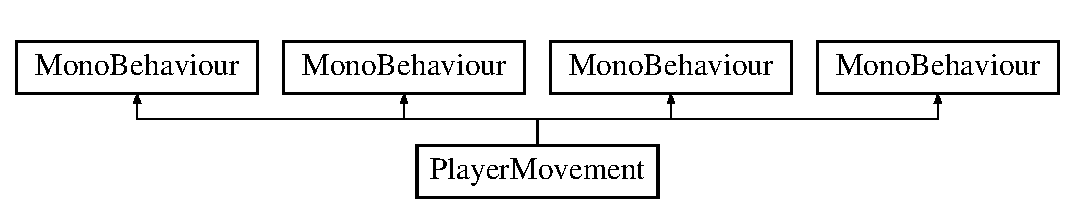
\includegraphics[height=2.000000cm]{class_player_movement}
\end{center}
\end{figure}
\subsection*{Public Member Functions}
\begin{DoxyCompactItemize}
\item 
void \mbox{\hyperlink{class_player_movement_abf3660ca2b1a352b4a9da98437c61aa3}{Start}} ()
\item 
void \mbox{\hyperlink{class_player_movement_aaf9b77d7177d538be9c1447d08191322}{Update}} ()
\item 
void \mbox{\hyperlink{class_player_movement_a0caaa871b9ef680c9f02bd0e22c77db1}{Fixed\+Update}} ()
\item 
void \mbox{\hyperlink{class_player_movement_aea65f5f7247feb09772da2543c8ec427}{Direction\+Switch}} ()
\end{DoxyCompactItemize}
\subsection*{Public Attributes}
\begin{DoxyCompactItemize}
\item 
\mbox{\Hypertarget{class_player_movement_aa83a2390fe399c816eac24ac74a02528}\label{class_player_movement_aa83a2390fe399c816eac24ac74a02528}} 
bool {\bfseries face\+Right} = true
\item 
\mbox{\Hypertarget{class_player_movement_aaf3e5c59c7392a57747a6a189c29febe}\label{class_player_movement_aaf3e5c59c7392a57747a6a189c29febe}} 
bool {\bfseries jump} = false
\item 
\mbox{\Hypertarget{class_player_movement_a411dc41a76270f4ff0ea15e0b996b8ed}\label{class_player_movement_a411dc41a76270f4ff0ea15e0b996b8ed}} 
float {\bfseries move\+Force} = 365f
\item 
\mbox{\Hypertarget{class_player_movement_a18b9bde59ef4f50acf685694f67ee3c7}\label{class_player_movement_a18b9bde59ef4f50acf685694f67ee3c7}} 
float {\bfseries max\+Speed} = 5f
\item 
\mbox{\Hypertarget{class_player_movement_a2918af247f8fd93a1dfe84b8d997c280}\label{class_player_movement_a2918af247f8fd93a1dfe84b8d997c280}} 
float {\bfseries jump\+Force} = 200f
\item 
\mbox{\Hypertarget{class_player_movement_a681e7b28ce40d859bbe21c231a676ce8}\label{class_player_movement_a681e7b28ce40d859bbe21c231a676ce8}} 
Transform {\bfseries ground\+Check}
\item 
\mbox{\Hypertarget{class_player_movement_a48a8923fa5137614141dd6886257af61}\label{class_player_movement_a48a8923fa5137614141dd6886257af61}} 
bool {\bfseries is\+Teleported} = false
\end{DoxyCompactItemize}


\subsection{Detailed Description}
Handles player movement. 

\subsection{Member Function Documentation}
\mbox{\Hypertarget{class_player_movement_aea65f5f7247feb09772da2543c8ec427}\label{class_player_movement_aea65f5f7247feb09772da2543c8ec427}} 
\index{Player\+Movement@{Player\+Movement}!Direction\+Switch@{Direction\+Switch}}
\index{Direction\+Switch@{Direction\+Switch}!Player\+Movement@{Player\+Movement}}
\subsubsection{\texorpdfstring{Direction\+Switch()}{DirectionSwitch()}}
{\footnotesize\ttfamily void Player\+Movement.\+Direction\+Switch (\begin{DoxyParamCaption}{ }\end{DoxyParamCaption})\hspace{0.3cm}{\ttfamily [inline]}}

Changes character direction. function is called by \mbox{\hyperlink{class_player_movement_a0caaa871b9ef680c9f02bd0e22c77db1}{Fixed\+Update()}} when user is switching direction of player \begin{DoxyPrecond}{Precondition}
User is pressing the left key 
\end{DoxyPrecond}
\begin{DoxyPostcond}{Postcondition}
Changes direction of the player if the left key is pressed 
\end{DoxyPostcond}
\mbox{\Hypertarget{class_player_movement_a0caaa871b9ef680c9f02bd0e22c77db1}\label{class_player_movement_a0caaa871b9ef680c9f02bd0e22c77db1}} 
\index{Player\+Movement@{Player\+Movement}!Fixed\+Update@{Fixed\+Update}}
\index{Fixed\+Update@{Fixed\+Update}!Player\+Movement@{Player\+Movement}}
\subsubsection{\texorpdfstring{Fixed\+Update()}{FixedUpdate()}}
{\footnotesize\ttfamily void Player\+Movement.\+Fixed\+Update (\begin{DoxyParamCaption}{ }\end{DoxyParamCaption})\hspace{0.3cm}{\ttfamily [inline]}}

Method is in charge of limiting the players moving speed and changing jump state if button is pressed. \begin{DoxyPrecond}{Precondition}
\mbox{\hyperlink{class_player_movement_aaf9b77d7177d538be9c1447d08191322}{Update()}} ran 
\end{DoxyPrecond}
\begin{DoxyPostcond}{Postcondition}
Movement of player is limited to our constraints 
\end{DoxyPostcond}
\mbox{\Hypertarget{class_player_movement_abf3660ca2b1a352b4a9da98437c61aa3}\label{class_player_movement_abf3660ca2b1a352b4a9da98437c61aa3}} 
\index{Player\+Movement@{Player\+Movement}!Start@{Start}}
\index{Start@{Start}!Player\+Movement@{Player\+Movement}}
\subsubsection{\texorpdfstring{Start()}{Start()}}
{\footnotesize\ttfamily void Player\+Movement.\+Start (\begin{DoxyParamCaption}{ }\end{DoxyParamCaption})\hspace{0.3cm}{\ttfamily [inline]}}

Runs at start. \begin{DoxyPrecond}{Precondition}
game starts 
\end{DoxyPrecond}
\begin{DoxyPostcond}{Postcondition}
Animator object and Rigidbody object get initialized for the player 
\end{DoxyPostcond}
\mbox{\Hypertarget{class_player_movement_aaf9b77d7177d538be9c1447d08191322}\label{class_player_movement_aaf9b77d7177d538be9c1447d08191322}} 
\index{Player\+Movement@{Player\+Movement}!Update@{Update}}
\index{Update@{Update}!Player\+Movement@{Player\+Movement}}
\subsubsection{\texorpdfstring{Update()}{Update()}}
{\footnotesize\ttfamily void Player\+Movement.\+Update (\begin{DoxyParamCaption}{ }\end{DoxyParamCaption})\hspace{0.3cm}{\ttfamily [inline]}}

Checks state of player every frame. \begin{DoxyPrecond}{Precondition}
none 
\end{DoxyPrecond}
\begin{DoxyPostcond}{Postcondition}
State of player gets changed depending on what was pressed 
\end{DoxyPostcond}


The documentation for this class was generated from the following file\+:\begin{DoxyCompactItemize}
\item 
Assets/\+Scripts/Player\+Movement.\+cs\end{DoxyCompactItemize}

\hypertarget{class_portal_movement}{}\section{Portal\+Movement Class Reference}
\label{class_portal_movement}\index{Portal\+Movement@{Portal\+Movement}}
Inheritance diagram for Portal\+Movement\+:\begin{figure}[H]
\begin{center}
\leavevmode
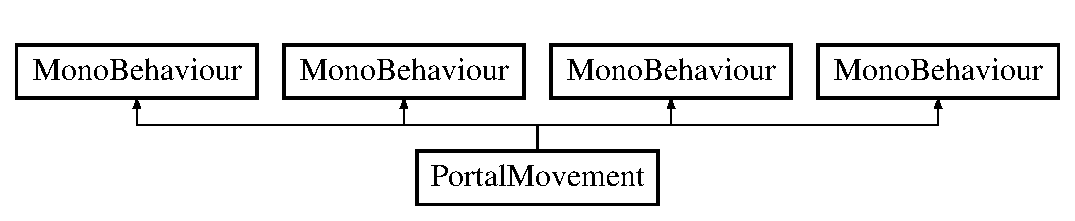
\includegraphics[height=2.000000cm]{class_portal_movement}
\end{center}
\end{figure}
\subsection*{Public Member Functions}
\begin{DoxyCompactItemize}
\item 
void \mbox{\hyperlink{class_portal_movement_aa7beca3afea663ec0de74142ac852ca4}{Start}} ()
\item 
\mbox{\Hypertarget{class_portal_movement_aeb23b9ab7c546f248da82c6e9b6dd473}\label{class_portal_movement_aeb23b9ab7c546f248da82c6e9b6dd473}} 
void {\bfseries Update} ()
\item 
void \mbox{\hyperlink{class_portal_movement_aa7beca3afea663ec0de74142ac852ca4}{Start}} ()
\item 
\mbox{\Hypertarget{class_portal_movement_aeb23b9ab7c546f248da82c6e9b6dd473}\label{class_portal_movement_aeb23b9ab7c546f248da82c6e9b6dd473}} 
void {\bfseries Update} ()
\end{DoxyCompactItemize}
\subsection*{Public Attributes}
\begin{DoxyCompactItemize}
\item 
\mbox{\Hypertarget{class_portal_movement_ad02d06d822cb837c2b6815bd0f448ca7}\label{class_portal_movement_ad02d06d822cb837c2b6815bd0f448ca7}} 
Vector2 {\bfseries target}
\item 
\mbox{\Hypertarget{class_portal_movement_a527ecae1396a95f37468482a7e717211}\label{class_portal_movement_a527ecae1396a95f37468482a7e717211}} 
Rigidbody2D {\bfseries rb}
\item 
\mbox{\Hypertarget{class_portal_movement_a206e9a3b0b782c6fd112bf99ff6a7bf4}\label{class_portal_movement_a206e9a3b0b782c6fd112bf99ff6a7bf4}} 
float {\bfseries speed} = 30f
\item 
\mbox{\Hypertarget{class_portal_movement_a80572fcf6a3158f6cc7fe64ed4d68f20}\label{class_portal_movement_a80572fcf6a3158f6cc7fe64ed4d68f20}} 
Vector2 {\bfseries move\+Direction}
\end{DoxyCompactItemize}


\subsection{Detailed Description}
Handles portal bullet movement. 

\subsection{Member Function Documentation}
\mbox{\Hypertarget{class_portal_movement_aa7beca3afea663ec0de74142ac852ca4}\label{class_portal_movement_aa7beca3afea663ec0de74142ac852ca4}} 
\index{Portal\+Movement@{Portal\+Movement}!Start@{Start}}
\index{Start@{Start}!Portal\+Movement@{Portal\+Movement}}
\subsubsection{\texorpdfstring{Start()}{Start()}\hspace{0.1cm}{\footnotesize\ttfamily [1/2]}}
{\footnotesize\ttfamily void Portal\+Movement.\+Start (\begin{DoxyParamCaption}{ }\end{DoxyParamCaption})\hspace{0.3cm}{\ttfamily [inline]}}

Method is in charge of the portal bullet movement. \begin{DoxyPrecond}{Precondition}
portal is shot 
\end{DoxyPrecond}
\begin{DoxyPostcond}{Postcondition}
portal bullet moves to the location of the mouse when it was clicked until it collides with a valid object 
\end{DoxyPostcond}
\mbox{\Hypertarget{class_portal_movement_aa7beca3afea663ec0de74142ac852ca4}\label{class_portal_movement_aa7beca3afea663ec0de74142ac852ca4}} 
\index{Portal\+Movement@{Portal\+Movement}!Start@{Start}}
\index{Start@{Start}!Portal\+Movement@{Portal\+Movement}}
\subsubsection{\texorpdfstring{Start()}{Start()}\hspace{0.1cm}{\footnotesize\ttfamily [2/2]}}
{\footnotesize\ttfamily void Portal\+Movement.\+Start (\begin{DoxyParamCaption}{ }\end{DoxyParamCaption})\hspace{0.3cm}{\ttfamily [inline]}}

Method is in charge of the portal bullet movement. \begin{DoxyPrecond}{Precondition}
portal is shot 
\end{DoxyPrecond}
\begin{DoxyPostcond}{Postcondition}
portal bullet moves to the location of the mouse when it was clicked until it collides with a valid object 
\end{DoxyPostcond}


The documentation for this class was generated from the following file\+:\begin{DoxyCompactItemize}
\item 
Assets/\+Scripts/Portal\+Movement.\+cs\end{DoxyCompactItemize}

\hypertarget{class_shoot_portal}{}\section{Shoot\+Portal Class Reference}
\label{class_shoot_portal}\index{Shoot\+Portal@{Shoot\+Portal}}
Inheritance diagram for Shoot\+Portal\+:\begin{figure}[H]
\begin{center}
\leavevmode
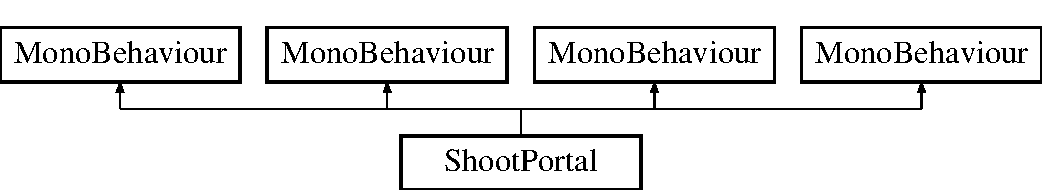
\includegraphics[height=2.000000cm]{class_shoot_portal}
\end{center}
\end{figure}
\subsection*{Public Member Functions}
\begin{DoxyCompactItemize}
\item 
\mbox{\Hypertarget{class_shoot_portal_afb543600d8358d399c285b327093a922}\label{class_shoot_portal_afb543600d8358d399c285b327093a922}} 
void {\bfseries Start} ()
\item 
void \mbox{\hyperlink{class_shoot_portal_a1160266ce719d6b93655286e0909bae8}{Update}} ()
\end{DoxyCompactItemize}
\subsection*{Public Attributes}
\begin{DoxyCompactItemize}
\item 
\mbox{\Hypertarget{class_shoot_portal_a715a70a24a5337424fc183a04cc0a3d2}\label{class_shoot_portal_a715a70a24a5337424fc183a04cc0a3d2}} 
Game\+Object {\bfseries blue\+Portal}
\item 
\mbox{\Hypertarget{class_shoot_portal_ad355d40bf4cc38c8deeb65c71c8b1d13}\label{class_shoot_portal_ad355d40bf4cc38c8deeb65c71c8b1d13}} 
Game\+Object {\bfseries red\+Portal}
\item 
\mbox{\Hypertarget{class_shoot_portal_ab1052b79920f7bdb495e3cc8af5d429d}\label{class_shoot_portal_ab1052b79920f7bdb495e3cc8af5d429d}} 
Vector2 {\bfseries velocity}
\end{DoxyCompactItemize}


\subsection{Detailed Description}
Handles portal shooting. 

\subsection{Member Function Documentation}
\mbox{\Hypertarget{class_shoot_portal_a1160266ce719d6b93655286e0909bae8}\label{class_shoot_portal_a1160266ce719d6b93655286e0909bae8}} 
\index{Shoot\+Portal@{Shoot\+Portal}!Update@{Update}}
\index{Update@{Update}!Shoot\+Portal@{Shoot\+Portal}}
\subsubsection{\texorpdfstring{Update()}{Update()}}
{\footnotesize\ttfamily void Shoot\+Portal.\+Update (\begin{DoxyParamCaption}{ }\end{DoxyParamCaption})\hspace{0.3cm}{\ttfamily [inline]}}

shoots a portal when mouse is clicked following the direction towards the location of the mouse pointer when clicked. \begin{DoxyPrecond}{Precondition}
mouse is clicked 
\end{DoxyPrecond}
\begin{DoxyPostcond}{Postcondition}
portal is shot 
\end{DoxyPostcond}


The documentation for this class was generated from the following file\+:\begin{DoxyCompactItemize}
\item 
Assets/\+Scripts/Shoot\+Portal.\+cs\end{DoxyCompactItemize}

\hypertarget{class_teleport_box}{}\section{Teleport\+Box Class Reference}
\label{class_teleport_box}\index{Teleport\+Box@{Teleport\+Box}}
Inheritance diagram for Teleport\+Box\+:\begin{figure}[H]
\begin{center}
\leavevmode
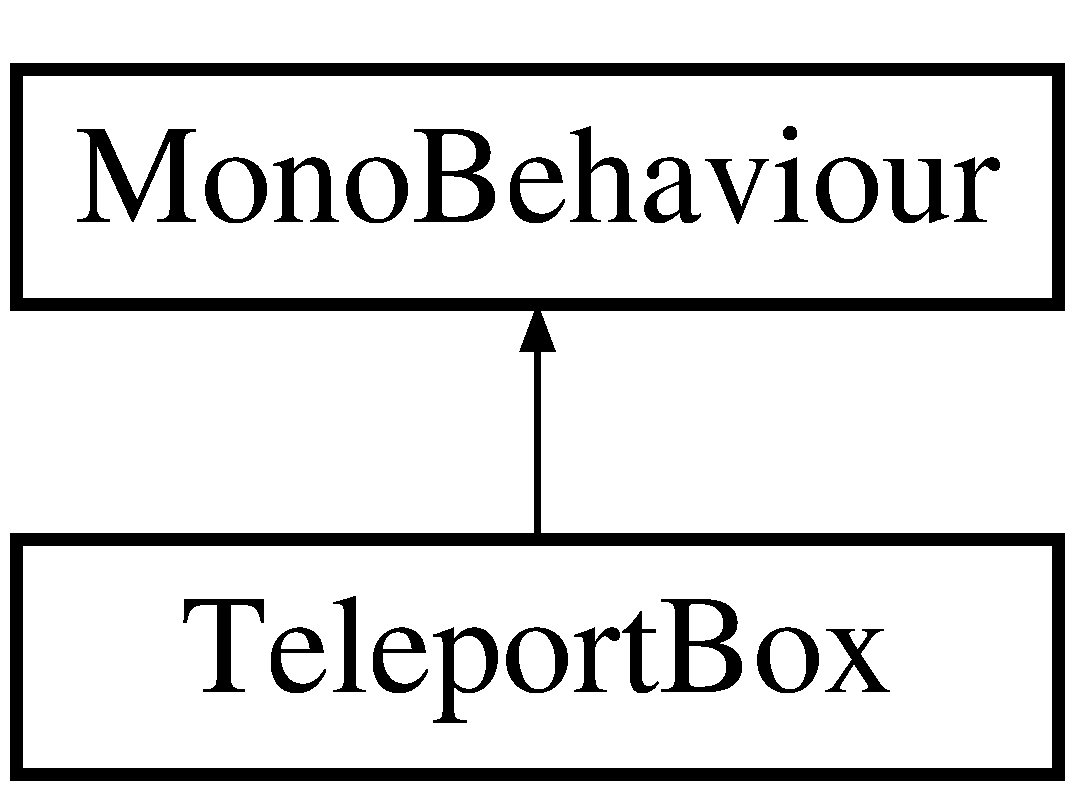
\includegraphics[height=2.000000cm]{class_teleport_box}
\end{center}
\end{figure}
\subsection*{Public Member Functions}
\begin{DoxyCompactItemize}
\item 
\mbox{\Hypertarget{class_teleport_box_a6e5afed61a3fae49c3e4cbf59845184f}\label{class_teleport_box_a6e5afed61a3fae49c3e4cbf59845184f}} 
void {\bfseries Start} ()
\item 
\mbox{\Hypertarget{class_teleport_box_ad4adb243e5c3307d1c2a634614e841de}\label{class_teleport_box_ad4adb243e5c3307d1c2a634614e841de}} 
void {\bfseries Update} ()
\item 
void \mbox{\hyperlink{class_teleport_box_ae75f32edd3ec30c3badd96e6d4c6cf31}{On\+Trigger\+Enter2D}} (Collider2D collision)
\item 
void \mbox{\hyperlink{class_teleport_box_ae10220f96d834813b63acce959fc009d}{On\+Trigger\+Exit2D}} (Collider2D collision)
\end{DoxyCompactItemize}
\subsection*{Public Attributes}
\begin{DoxyCompactItemize}
\item 
\mbox{\Hypertarget{class_teleport_box_aded6e64d463b8cac6fcc2727831c66ed}\label{class_teleport_box_aded6e64d463b8cac6fcc2727831c66ed}} 
string {\bfseries portal\+Entered}
\end{DoxyCompactItemize}


\subsection{Member Function Documentation}
\mbox{\Hypertarget{class_teleport_box_ae75f32edd3ec30c3badd96e6d4c6cf31}\label{class_teleport_box_ae75f32edd3ec30c3badd96e6d4c6cf31}} 
\index{Teleport\+Box@{Teleport\+Box}!On\+Trigger\+Enter2D@{On\+Trigger\+Enter2D}}
\index{On\+Trigger\+Enter2D@{On\+Trigger\+Enter2D}!Teleport\+Box@{Teleport\+Box}}
\subsubsection{\texorpdfstring{On\+Trigger\+Enter2\+D()}{OnTriggerEnter2D()}}
{\footnotesize\ttfamily void Teleport\+Box.\+On\+Trigger\+Enter2D (\begin{DoxyParamCaption}\item[{Collider2D}]{collision }\end{DoxyParamCaption})\hspace{0.3cm}{\ttfamily [inline]}}

This method runs after registering collision of box with portal and its goal is to switch the position of the box to that one of the other portal \begin{DoxyPrecond}{Precondition}
portals are created within an appropiate surface 
\end{DoxyPrecond}
\begin{DoxyPostcond}{Postcondition}
after box enters a portal it\textquotesingle{}s position changes to that of the other portal 
\end{DoxyPostcond}

\begin{DoxyParams}{Parameters}
{\em collision} & collision object created by the physics engine \\
\hline
\end{DoxyParams}
\mbox{\Hypertarget{class_teleport_box_ae10220f96d834813b63acce959fc009d}\label{class_teleport_box_ae10220f96d834813b63acce959fc009d}} 
\index{Teleport\+Box@{Teleport\+Box}!On\+Trigger\+Exit2D@{On\+Trigger\+Exit2D}}
\index{On\+Trigger\+Exit2D@{On\+Trigger\+Exit2D}!Teleport\+Box@{Teleport\+Box}}
\subsubsection{\texorpdfstring{On\+Trigger\+Exit2\+D()}{OnTriggerExit2D()}}
{\footnotesize\ttfamily void Teleport\+Box.\+On\+Trigger\+Exit2D (\begin{DoxyParamCaption}\item[{Collider2D}]{collision }\end{DoxyParamCaption})\hspace{0.3cm}{\ttfamily [inline]}}

Resets the state of the box after its position is changed between the portals 
\begin{DoxyParams}{Parameters}
{\em collision} & collision object created by the physics engine \\
\hline
\end{DoxyParams}


The documentation for this class was generated from the following file\+:\begin{DoxyCompactItemize}
\item 
Assets/\+Scripts/Teleport\+Box.\+cs\end{DoxyCompactItemize}

\hypertarget{classteleporter_location}{}\section{teleporter\+Location Class Reference}
\label{classteleporter_location}\index{teleporter\+Location@{teleporter\+Location}}
Inheritance diagram for teleporter\+Location\+:\begin{figure}[H]
\begin{center}
\leavevmode
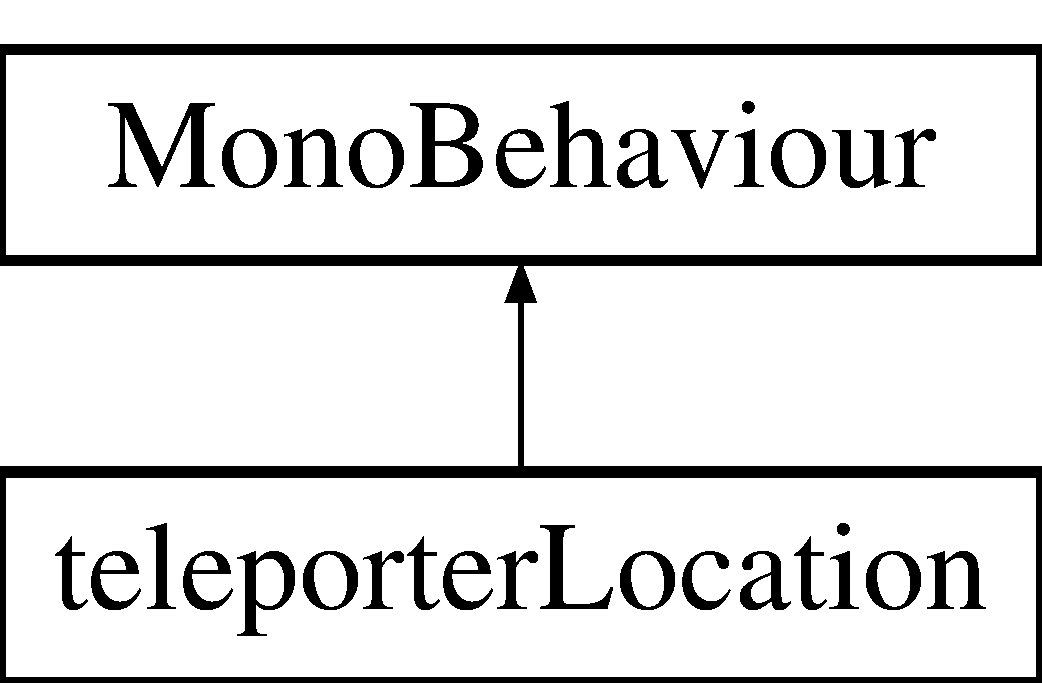
\includegraphics[height=2.000000cm]{classteleporter_location}
\end{center}
\end{figure}
\subsection*{Public Attributes}
\begin{DoxyCompactItemize}
\item 
\mbox{\Hypertarget{classteleporter_location_a772d1224edea45e9a7ee52c35562fd7c}\label{classteleporter_location_a772d1224edea45e9a7ee52c35562fd7c}} 
string {\bfseries location}
\end{DoxyCompactItemize}


The documentation for this class was generated from the following file\+:\begin{DoxyCompactItemize}
\item 
Assets/\+Scripts/teleporter\+Location.\+cs\end{DoxyCompactItemize}

\hypertarget{class_teleport_player}{}\section{Teleport\+Player Class Reference}
\label{class_teleport_player}\index{Teleport\+Player@{Teleport\+Player}}
Inheritance diagram for Teleport\+Player\+:\begin{figure}[H]
\begin{center}
\leavevmode
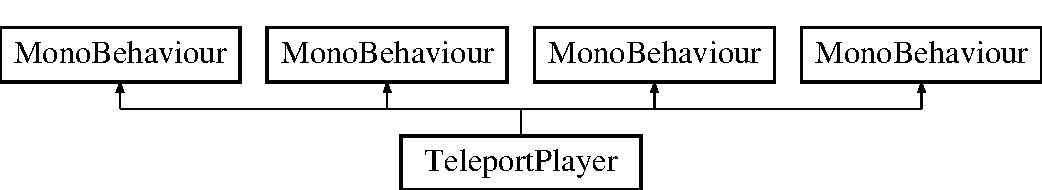
\includegraphics[height=2.000000cm]{class_teleport_player}
\end{center}
\end{figure}
\subsection*{Public Member Functions}
\begin{DoxyCompactItemize}
\item 
void \mbox{\hyperlink{class_teleport_player_a555b0c226c512d6bc9ce347b19957cd9}{On\+Trigger\+Enter2D}} (Collider2D collision)
\item 
void \mbox{\hyperlink{class_teleport_player_addd6af261867cf134ac87c580cebec92}{On\+Trigger\+Exit2D}} (Collider2D collision)
\item 
\mbox{\Hypertarget{class_teleport_player_ad75d1699964434878bf8a31244a6a4af}\label{class_teleport_player_ad75d1699964434878bf8a31244a6a4af}} 
void {\bfseries Start} ()
\item 
\mbox{\Hypertarget{class_teleport_player_ab8dc957d5f4ca8e3bee2d4b48ac0ed23}\label{class_teleport_player_ab8dc957d5f4ca8e3bee2d4b48ac0ed23}} 
void {\bfseries Update} ()
\item 
void \mbox{\hyperlink{class_teleport_player_a1ab94b6c3d13f1287f9127393afe2298}{On\+Collision\+Enter2D}} (Collision2D collision)
\item 
void \mbox{\hyperlink{class_teleport_player_ac85fc2322d2dc27de518434422c2c25e}{On\+Collision\+Exit2D}} (Collision2D collision)
\end{DoxyCompactItemize}
\subsection*{Public Attributes}
\begin{DoxyCompactItemize}
\item 
\mbox{\Hypertarget{class_teleport_player_a3a1f027838b709b22b058dd5d8a4a140}\label{class_teleport_player_a3a1f027838b709b22b058dd5d8a4a140}} 
string {\bfseries portal\+Entered}
\end{DoxyCompactItemize}


\subsection{Detailed Description}
Handles player teleporting

Handles teleporting players between portals. 

\subsection{Member Function Documentation}
\mbox{\Hypertarget{class_teleport_player_a1ab94b6c3d13f1287f9127393afe2298}\label{class_teleport_player_a1ab94b6c3d13f1287f9127393afe2298}} 
\index{Teleport\+Player@{Teleport\+Player}!On\+Collision\+Enter2D@{On\+Collision\+Enter2D}}
\index{On\+Collision\+Enter2D@{On\+Collision\+Enter2D}!Teleport\+Player@{Teleport\+Player}}
\subsubsection{\texorpdfstring{On\+Collision\+Enter2\+D()}{OnCollisionEnter2D()}}
{\footnotesize\ttfamily void Teleport\+Player.\+On\+Collision\+Enter2D (\begin{DoxyParamCaption}\item[{Collision2D}]{collision }\end{DoxyParamCaption})\hspace{0.3cm}{\ttfamily [inline]}}

This method runs after registering collision of player with portal and its goal is to switch the position of the player to that one of the other portal. pre\+: portals are created within an appropiate surface post\+: after player enters a portal it\textquotesingle{}s position changes to that of the other portal \mbox{\Hypertarget{class_teleport_player_ac85fc2322d2dc27de518434422c2c25e}\label{class_teleport_player_ac85fc2322d2dc27de518434422c2c25e}} 
\index{Teleport\+Player@{Teleport\+Player}!On\+Collision\+Exit2D@{On\+Collision\+Exit2D}}
\index{On\+Collision\+Exit2D@{On\+Collision\+Exit2D}!Teleport\+Player@{Teleport\+Player}}
\subsubsection{\texorpdfstring{On\+Collision\+Exit2\+D()}{OnCollisionExit2D()}}
{\footnotesize\ttfamily void Teleport\+Player.\+On\+Collision\+Exit2D (\begin{DoxyParamCaption}\item[{Collision2D}]{collision }\end{DoxyParamCaption})\hspace{0.3cm}{\ttfamily [inline]}}

Resets the state of the player after its position is changed between the portals. \mbox{\Hypertarget{class_teleport_player_a555b0c226c512d6bc9ce347b19957cd9}\label{class_teleport_player_a555b0c226c512d6bc9ce347b19957cd9}} 
\index{Teleport\+Player@{Teleport\+Player}!On\+Trigger\+Enter2D@{On\+Trigger\+Enter2D}}
\index{On\+Trigger\+Enter2D@{On\+Trigger\+Enter2D}!Teleport\+Player@{Teleport\+Player}}
\subsubsection{\texorpdfstring{On\+Trigger\+Enter2\+D()}{OnTriggerEnter2D()}}
{\footnotesize\ttfamily void Teleport\+Player.\+On\+Trigger\+Enter2D (\begin{DoxyParamCaption}\item[{Collider2D}]{collision }\end{DoxyParamCaption})\hspace{0.3cm}{\ttfamily [inline]}}

This method runs after registering collision of player with portal and its goal is to switch the position of the player to that one of the other portal \begin{DoxyPrecond}{Precondition}
portals are created within an appropiate surface 
\end{DoxyPrecond}
\begin{DoxyPostcond}{Postcondition}
after player enters a portal it\textquotesingle{}s position changes to that of the other portal 
\end{DoxyPostcond}

\begin{DoxyParams}{Parameters}
{\em collision} & collision object created by the physics engine \\
\hline
\end{DoxyParams}
\mbox{\Hypertarget{class_teleport_player_addd6af261867cf134ac87c580cebec92}\label{class_teleport_player_addd6af261867cf134ac87c580cebec92}} 
\index{Teleport\+Player@{Teleport\+Player}!On\+Trigger\+Exit2D@{On\+Trigger\+Exit2D}}
\index{On\+Trigger\+Exit2D@{On\+Trigger\+Exit2D}!Teleport\+Player@{Teleport\+Player}}
\subsubsection{\texorpdfstring{On\+Trigger\+Exit2\+D()}{OnTriggerExit2D()}}
{\footnotesize\ttfamily void Teleport\+Player.\+On\+Trigger\+Exit2D (\begin{DoxyParamCaption}\item[{Collider2D}]{collision }\end{DoxyParamCaption})\hspace{0.3cm}{\ttfamily [inline]}}

Resets the state of the player after its position is changed between the portals 
\begin{DoxyParams}{Parameters}
{\em collision} & collision object created by the physics engine \\
\hline
\end{DoxyParams}


The documentation for this class was generated from the following file\+:\begin{DoxyCompactItemize}
\item 
Assets/\+Scripts/Teleport\+Player.\+cs\end{DoxyCompactItemize}

\hypertarget{class_win_game}{}\section{Win\+Game Class Reference}
\label{class_win_game}\index{Win\+Game@{Win\+Game}}
Inheritance diagram for Win\+Game\+:\begin{figure}[H]
\begin{center}
\leavevmode
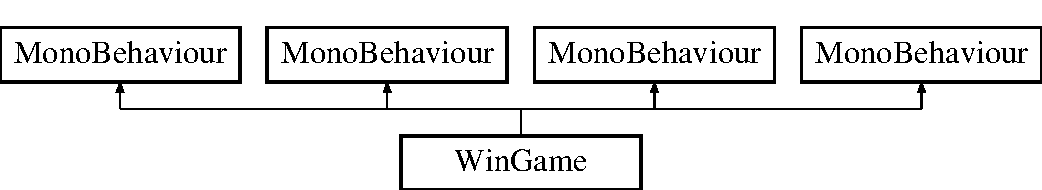
\includegraphics[height=2.000000cm]{class_win_game}
\end{center}
\end{figure}
\subsection*{Public Member Functions}
\begin{DoxyCompactItemize}
\item 
void \mbox{\hyperlink{class_win_game_a20f3871fd050c6da54d041b49a7fb063}{On\+Collision\+Enter2D}} (Collision2D collision)
\item 
void \mbox{\hyperlink{class_win_game_a20f3871fd050c6da54d041b49a7fb063}{On\+Collision\+Enter2D}} (Collision2D collision)
\end{DoxyCompactItemize}
\subsection*{Public Attributes}
\begin{DoxyCompactItemize}
\item 
\mbox{\Hypertarget{class_win_game_a786a1f699b803e4eafe16804002e4f18}\label{class_win_game_a786a1f699b803e4eafe16804002e4f18}} 
Game\+Object {\bfseries you\+Win}
\end{DoxyCompactItemize}


\subsection{Detailed Description}
Handles completion of level. 

\subsection{Member Function Documentation}
\mbox{\Hypertarget{class_win_game_a20f3871fd050c6da54d041b49a7fb063}\label{class_win_game_a20f3871fd050c6da54d041b49a7fb063}} 
\index{Win\+Game@{Win\+Game}!On\+Collision\+Enter2D@{On\+Collision\+Enter2D}}
\index{On\+Collision\+Enter2D@{On\+Collision\+Enter2D}!Win\+Game@{Win\+Game}}
\subsubsection{\texorpdfstring{On\+Collision\+Enter2\+D()}{OnCollisionEnter2D()}\hspace{0.1cm}{\footnotesize\ttfamily [1/2]}}
{\footnotesize\ttfamily void Win\+Game.\+On\+Collision\+Enter2D (\begin{DoxyParamCaption}\item[{Collision2D}]{collision }\end{DoxyParamCaption})\hspace{0.3cm}{\ttfamily [inline]}}

Sets win state to true. \begin{DoxyPrecond}{Precondition}
Player reaches the door object 
\end{DoxyPrecond}
\begin{DoxyPostcond}{Postcondition}
Success message is displayed indicating level completed After Player \char`\"{}collides\char`\"{} with door object it will display a Win message indicating level completion 
\end{DoxyPostcond}
\mbox{\Hypertarget{class_win_game_a20f3871fd050c6da54d041b49a7fb063}\label{class_win_game_a20f3871fd050c6da54d041b49a7fb063}} 
\index{Win\+Game@{Win\+Game}!On\+Collision\+Enter2D@{On\+Collision\+Enter2D}}
\index{On\+Collision\+Enter2D@{On\+Collision\+Enter2D}!Win\+Game@{Win\+Game}}
\subsubsection{\texorpdfstring{On\+Collision\+Enter2\+D()}{OnCollisionEnter2D()}\hspace{0.1cm}{\footnotesize\ttfamily [2/2]}}
{\footnotesize\ttfamily void Win\+Game.\+On\+Collision\+Enter2D (\begin{DoxyParamCaption}\item[{Collision2D}]{collision }\end{DoxyParamCaption})\hspace{0.3cm}{\ttfamily [inline]}}

Sets win state to true. \begin{DoxyPrecond}{Precondition}
Player reaches the door object 
\end{DoxyPrecond}
\begin{DoxyPostcond}{Postcondition}
Success message is displayed indicating level completed After Player \char`\"{}collides\char`\"{} with door object it will display a Win message indicating level completion 
\end{DoxyPostcond}

\begin{DoxyParams}{Parameters}
{\em collision} & collision object created by the physics engine \\
\hline
\end{DoxyParams}


The documentation for this class was generated from the following file\+:\begin{DoxyCompactItemize}
\item 
Assets/\+Scripts/Win\+Game.\+cs\end{DoxyCompactItemize}

%--- End generated contents ---

% Index
\backmatter
\newpage
\phantomsection
\clearemptydoublepage
\addcontentsline{toc}{chapter}{Index}
\printindex

\end{document}
